\documentclass[12pt, a4paper]{article}


% --- 核心宏包 ---
\usepackage{graphics}
\usepackage{float}
\usepackage[UTF8]{ctex}        % 中文支持
\usepackage{geometry}         % 页面边距
\usepackage{graphicx}         % 插入图片
\usepackage{amsmath, amssymb} % 数学公式
\usepackage{setspace}         % 行间距
\usepackage{titlesec}         % 标题格式定制
\usepackage{booktabs}         % 三线表
\usepackage{hyperref}         % 超链接
\usepackage{multirow}         % 多行表格
\usepackage{array}            % 表格列格式
\usepackage{listings}         % 代码高亮
\usepackage{xcolor}           % 颜色
\usepackage[backend=biber, style=gb7714-2015]{biblatex}
\addbibresource{refs.bib}

% --- 页面设置 ---
\geometry{left=3.18cm, right=3.18cm, top=2.54cm, bottom=2.54cm}
\onehalfspacing

% --- 标题格式设置 ---
\titleformat{\section}{\large\bfseries}{\thesection}{1em}{}
\titleformat{\subsection}{\normalsize\bfseries}{\thesubsection}{1em}{}
\titleformat{\subsubsection}{\normalsize\bfseries}{\thesubsubsection}{1em}{}

% --- 代码环境 ---
\lstset{
  basicstyle=\small\ttfamily,
  keywordstyle=\color{blue},
  commentstyle=\color{gray},
  numbers=left,
  numberstyle=\tiny\color{gray},
  frame=single,
  breaklines=true,
  captionpos=b
}

\begin{document}

% --- 封面 ---
\begin{center}
	
\includegraphics[width=0.8\textwidth]{figures/XJTU_2024.png}
	\vspace*{1.5cm}
	\newline
	{\LARGE \textbf{面向边缘智能应用的低功耗Int8数字存算一体架构设计及FPGA验证}} \\[2cm]

	\vspace*{3cm}

	\begin{spacing}{2.0}
		\begin{tabular}{ll}
			\textbf{学 \quad 号：} & 2221411116                                                                   \\
			\textbf{姓 \quad 名：} & 焦宏宝                                                                          \\
			\textbf{导 \quad 师：} & 梁峰                                                                           \\
			\textbf{论文题目：}      & \begin{tabular}[t]{l} 面向边缘智能应用的低功耗Int8 -- \\ 数字存算一体架构设计及FPGA验证 \end{tabular} \\
			\textbf{专 \quad 业：} & 微电子科学与工程 强芯实验班                                                               \\
			\textbf{学 \quad 院：} & 电信学部　微电子学院                                                                   \\
			\textbf{填写时间：}      & 2026年 04月
		\end{tabular}
	\end{spacing}
\end{center}

\newpage

% --- 摘要 ---
\begin{center}
	{\large\bfseries 摘\quad 要}
\end{center}

随着深度学习在边缘智能场景中的广泛部署，传统冯·诺依曼架构中处理器与存储器分离所带来的数据搬运瓶颈日益突出。存算一体（Computing-in-Memory, CIM）技术通过在存储阵列内部或近存储位置完成计算，从体系结构层面缓解"内存墙"问题，被认为是提升推理能效与吞吐率的重要方向。

本文设计并实现了一种面向边缘推理的低功耗INT8数字存算一体矩阵计算阵列架构。系统以16×16 CIM Tile为原子计算单元，采用参数化设计支持可配置并行度，核心引擎通过7级流水线状态机实现权重加载、零点减法、MAC运算、偏置累加、ReLU激活、重量化与结果写回的完整推理数据通路。权重存储采用16-bank SRAM拆分架构以确保Vivado BRAM推断，并通过AXI4-Lite接口实现DMA式权重写入与CSR运行时配置。

在软核控制方面，集成了PicoRV32 RISC-V软核替代ARM PS进行推理控制，通过Wishbone-to-CSR桥接实现与CIM IP完全相同的AXI事务，配合双端口BRAM实现运行时固件加载与结果回读，使CIM加速器可在纯PL侧自主运行。

本设计在PYNQ-Z2（Zynq-7020）平台完成综合部署与板级验证。ARM控制模式下，MLP网络（784→128→10）以60 MHz工作频率实现单幅推理3282周期，LeNet-5 CNN（7层）实现76034周期，20张MNIST手写数字图片上分类准确率100\%（模型在完整测试集上约93\%），200张图片上准确率99.5\%，全部输出与Python bit-accurate参考模型逐元素一致。PicoRV32模式以50 MHz时序收敛，增加仅1627个LUT与9个BRAM的开销，200张MNIST图片验证准确率96.5\%，全部logits与ARM控制路径bit-exact一致。相对ARM Cortex-A9纯NumPy基线，MLP推理加速比约25.8倍，LeNet-5加速比约20.9倍（sequential逐像素模式对比）。系统占用LUT 20.84\%、BRAM 25\%、DSP 100\%（220个），CIM IP动态功耗仅0.284 W。

\vspace{1em}
\noindent\textbf{关键词：}存算一体；INT8量化推理；FPGA验证；CIM阵列；PicoRV32；PYNQ-Z2

\newpage

% --- Abstract ---
\begin{center}
	{\large\bfseries Abstract}
\end{center}

With the widespread deployment of deep learning at the edge, the data movement bottleneck caused by the separation of processor and memory in traditional von Neumann architectures has become increasingly prominent. Computing-in-Memory (CIM) technology mitigates the "memory wall" problem at the architectural level by performing computation within or near memory arrays, and is considered a promising direction for improving inference energy efficiency and throughput.

This thesis designs and implements a low-power INT8 digital computing-in-memory matrix computation array architecture for edge inference. The system employs a 16×16 CIM Tile as the atomic compute unit with parameterized parallelism. The core engine implements a 7-stage pipelined FSM covering the complete inference datapath: weight loading, zero-point subtraction, MAC operation, bias accumulation, ReLU activation, requantization, and result writeback. Weight storage uses a 16-bank SRAM split architecture for reliable Vivado BRAM inference, with an AXI4-Lite interface for DMA-style weight loading and runtime CSR configuration.

For soft-core control, a PicoRV32 RISC-V core is integrated to replace ARM PS for inference control, using a Wishbone-to-CSR bridge that issues the same AXI transactions as the ARM path, with dual-port BRAMs for runtime firmware loading and result readback.

The design is synthesized and verified on a PYNQ-Z2 (Zynq-7020) platform. Under ARM control at 60 MHz, the MLP network (784→128→10) achieves 3282 cycles per inference, and LeNet-5 CNN (7 layers) achieves 76034 cycles, achieving 100\% classification accuracy on 20 test images (model accuracy $\sim$93\% on the full MNIST test set) and 99.5\% on 200 test images respectively, all outputs bit-exact with the Python golden model. The PicoRV32 mode achieves timing closure at 50 MHz with only 1627 additional LUTs and 9 BRAMs, validated on 200 MNIST images with 96.5\% accuracy and 100\% bit-exact logits. Compared to a NumPy baseline on ARM Cortex-A9, the CIM hardware achieves approximately 25.8$\times$ speedup for MLP and 20.9$\times$ for LeNet-5 (sequential per-pixel comparison). The system utilizes 20.84\% LUTs, 25\% BRAM, 100\% DSP (220 units), with the CIM IP consuming only 0.284 W dynamic power.

\vspace{1em}
\noindent\textbf{Keywords:} Computing-in-Memory; INT8 quantized inference; FPGA verification; CIM array; PicoRV32; PYNQ-Z2

\newpage

% --- 目录 ---
\tableofcontents
\newpage

% ====================================================================
\section{绪论}
% ====================================================================

\subsection{选题背景}

近年来，以YOLO\cite{10}、SSD\cite{11}为代表的深度学习目标检测算法在智能安防、工业视觉、无人系统与车载感知等场景中被广泛采用，其共同特点是需要在较高精度下实现接近实时的推理能力，而网络内部又以卷积/矩阵乘加（MAC）为主导计算负载，导致整体计算量与数据访问量都十分庞大。YOLO将检测任务端到端地建模为单网络回归问题，SSD通过多尺度特征图上的卷积预测实现单阶段检测，这类方法在追求速度与精度的同时，也使得卷积算子成为系统性能与功耗优化的核心瓶颈之一。

\begin{figure}[H]
	\centering
	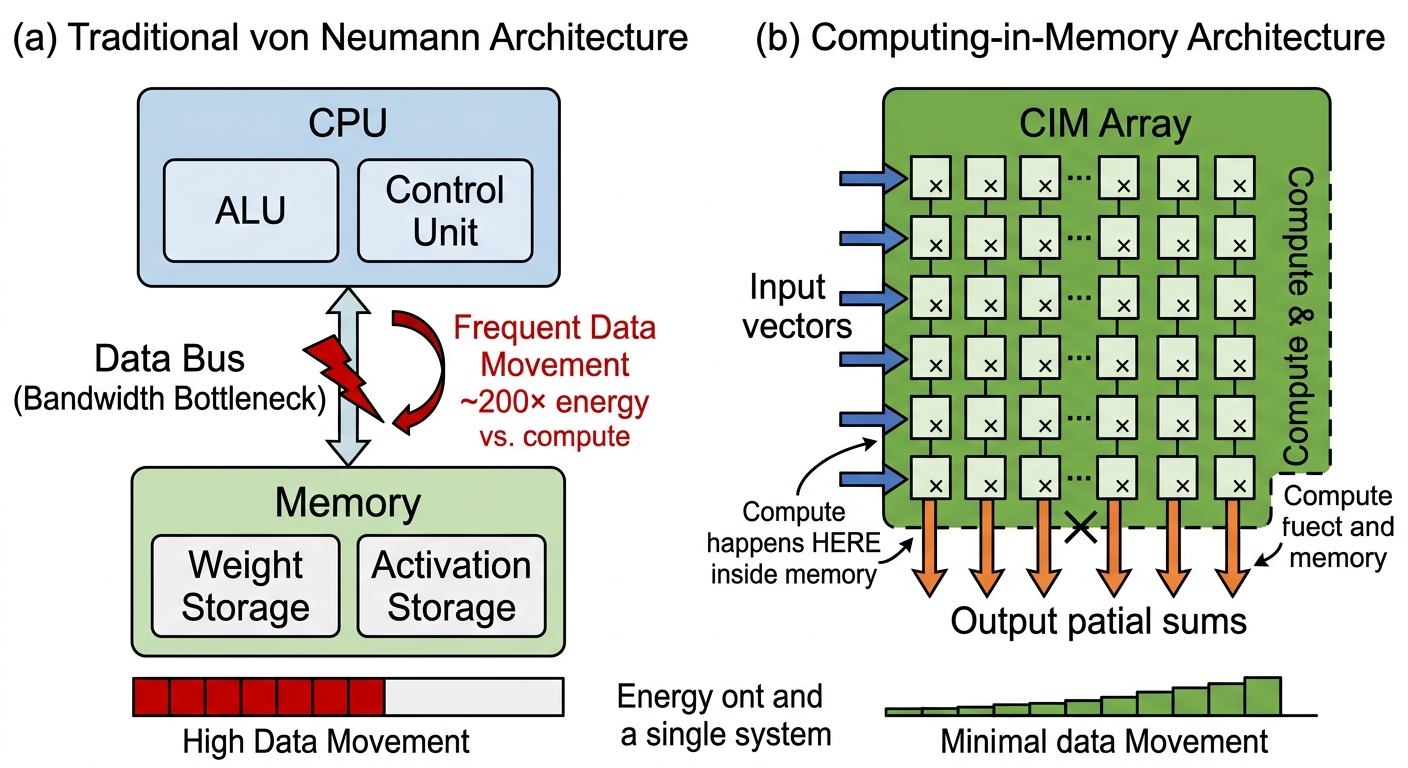
\includegraphics[width=0.85\textwidth]{figures/m1.png}
	\caption{传统冯·诺依曼架构与存算一体架构对比}
	\label{fig:vonneumann_vs_cim}
\end{figure}

然而，在传统冯·诺依曼架构中，处理器与存储器相互分离，权重与特征图等数据需要在存储层级与计算单元之间频繁搬运，系统性能逐渐受限于存储带宽与访问延迟，"内存墙（Memory Wall）"问题由此形成并长期存在（如图\ref{fig:vonneumann_vs_cim}所示）。Wulf与McKee早在1995年就指出处理器速度提升与存储器速度提升之间的差距会不断扩大，从而限制系统级性能提升\cite{1}。与此同时，能效维度的矛盾更加突出：在先进工艺条件下，数据搬运（尤其是跨层级、跨片外存储访问）相对于算术运算存在显著更高的能量代价，使得"算得快"并不等价于"算得省"。Horowitz在ISSCC 2014的报告中系统讨论了计算系统的能耗拆分，强调需要从体系结构与数据流层面减少昂贵的数据访问\cite{2}。面向CNN的专用加速器研究也进一步表明：通过数据复用与数据流优化降低（尤其是片外）访存开销，是实现低功耗实时推理的关键路径之一\cite{3}。在边缘计算场景（电池供电、散热受限、实时性要求高）中，上述矛盾更加尖锐，传统"分离式计算-存储"模式难以同时满足吞吐与能效需求。

存算一体（Computing-in-Memory, CIM）技术通过在存储阵列内部或近存储位置完成计算，将"数据搬运"转化为"原位计算"，从体系结构层面缓解冯·诺依曼瓶颈，被认为是突破内存墙、提升能效与吞吐率的重要方向。Nature Electronics的综述工作提出了覆盖不同存储器参与程度的CIM全谱系分类框架，并指出CIM可在逻辑运算与乘加运算等基本原语上实现能效提升\cite{4}。在诸多实现路径中，基于标准CMOS工艺的SRAM-CIM具有速度快、工艺成熟、可靠性高、与主流数字设计流程兼容等优点，是面向工程落地与系统集成的重要路线之一\cite{5}。

从应用角度看，为在精度、硬件复杂度与系统吞吐之间取得平衡，Int8量化推理已成为工业界与学术界常用的落地方案之一。Jacob等人提出的整数算术推理量化方法表明，通过合理的量化尺度与训练/校准策略，可在保持精度的前提下实现高效的整数运算推理流程\cite{6}。从硬件角度看，已有研究在SRAM-CIM宏单元中展示了面向多比特MAC的实现范式，如8b MAC的SRAM CIM宏以及支持Signed-INT8的SRAM CIM宏等工作，说明"多比特、可用于实际推理精度需求"的SRAM-CIM在工程上具有可行性\cite{8}。

基于上述背景，本课题面向边缘智能推理的能效与实时性需求，在标准CMOS SRAM工艺假设下，设计了一种支持Int8数据类型的数字存算一体矩阵计算阵列架构（设计空间定位与两种实现极端的分析见§\ref{sec:two_extremes}）：在存储阵列内实现权重存储与乘法/部分积生成，结合合理的阵列并行组织、累加与数据通路调度，降低数据搬运开销并提升并行吞吐；同时采用SystemVerilog完成RTL级实现，并在FPGA平台完成综合部署与功能验证，形成了可复现的验证平台与完整代码交付。

\subsection{国内外现状及发展趋势}

存算一体研究近年来快速发展，已形成覆盖器件/电路/架构/算法的多层次技术体系。相关综述工作从实现介质（SRAM、DRAM、RRAM/PCM等）与计算形态（模拟/数字、阵列内/近存储）对CIM进行系统分类（如图\ref{fig:cim_taxonomy}所示），指出其共同目标是减少访存与数据移动开销、利用阵列并行提升吞吐\cite{4}\cite{5}\cite{12}\cite{14}。

在国际研究中，基于新型非易失存储器（如RRAM）交叉阵列的模拟CIM方案曾是重要热点，典型代表包括ISAAC\cite{17}和PRIME\cite{18}等工作。PUMA等可编程memristor加速器进一步探索了更可编程的推理加速路径\cite{19}。但模拟CIM往往需要ADC/DAC等外围电路并面临器件非理想性、噪声、精度与可校准性等挑战\cite{4}\cite{15}。面向通用存储体系的近存储计算也形成了多条路线，如Ambit\cite{21}、Neural Cache\cite{20}、FloatPIM\cite{22}等。

在电路与工程实现层面，基于标准CMOS工艺的SRAM-CIM因其速度、成熟度与数字设计流程兼容性而成为当前研究与产业化的重要路线\cite{5}\cite{12}\cite{14}。已有多项芯片级宏单元工作给出了可参考的实现范式，如28nm工艺下实现8b MAC的SRAM-CIM宏单元，以及支持Signed-INT8的ADC-less SRAM-CIM宏单元\cite{8}。研究趋势正从"单个CIM宏单元验证"走向"可重构/可编程的数字CIM处理器与系统级加速器"。Tu等报道了支持BF16与INT8的可重构数字CIM处理器\cite{24}，其后续ReDCIM工作给出了统一FP/INT的数字CIM设计\cite{25}。同期也出现面向Transformer/注意力工作负载的数字CIM加速研究，如TranCIM\cite{26}、MulTCIM\cite{27}等。

在算法侧，Int8量化推理已成为常用的落地路径。Jacob等工作提出的整数算术推理量化方法提供了硬件采用Int8数据通路的算法依据\cite{6}。PACT\cite{28}与LSQ\cite{29}等研究进一步从训练与量化参数学习角度改善量化精度。

综合来看，国内外CIM研究呈现如下趋势：技术路线从"模拟/新型器件主导"扩展为"模拟与全数字并行发展"；算子与精度从低比特走向多比特MAC（尤其是Signed-INT8）；应用从CNN拓展到Transformer/多模态；验证方式越来越需要体系结构层面的可复现评估（包括RTL/FPGA原型验证、资源/频率/吞吐/延迟评估等）\cite{12}\cite{16}。本课题正是在此背景下，以数字SRAM-CIM阵列架构为核心，围绕数据通路、控制调度与FPGA验证建立了工程闭环。

\begin{figure}[H]
	\centering
	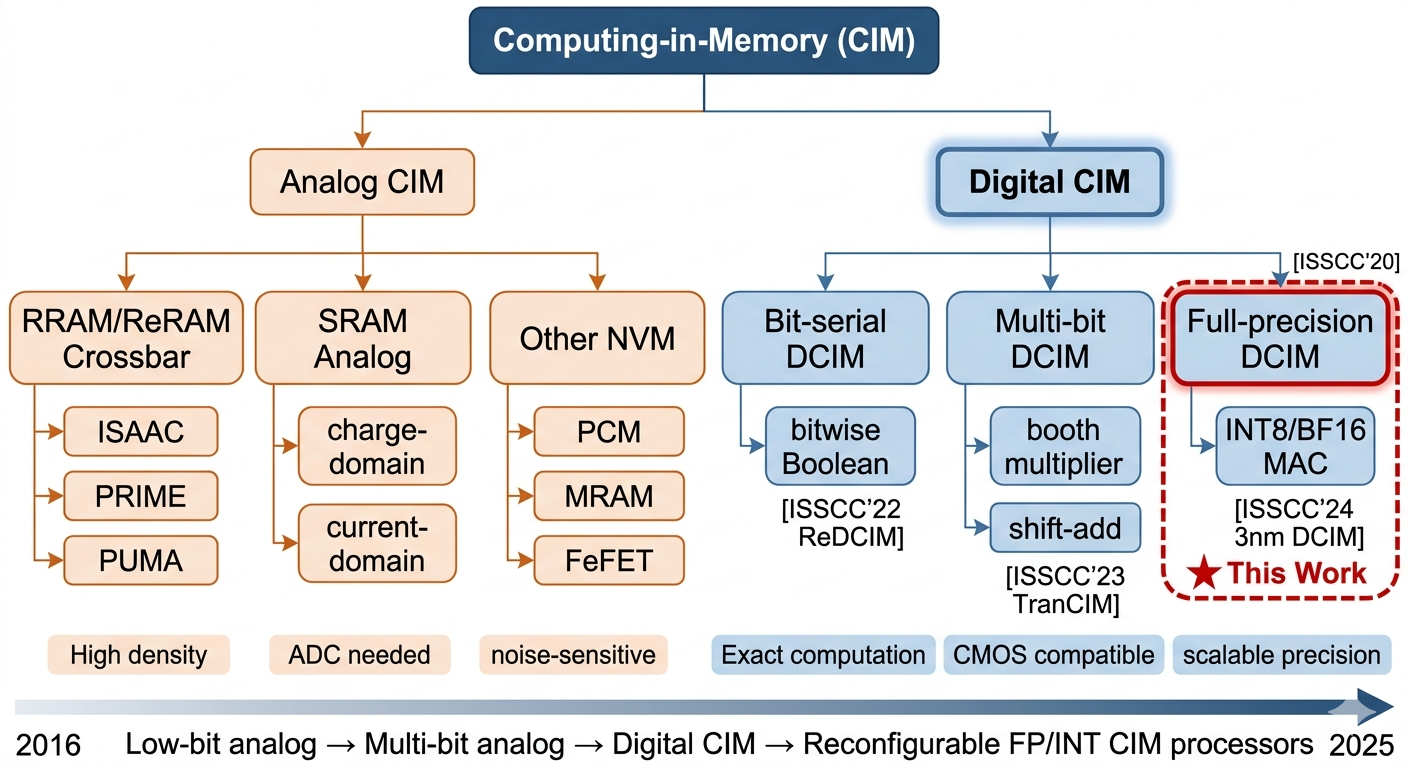
\includegraphics[width=0.85\textwidth]{figures/m2.png}
	\caption{CIM技术全谱系分类框架与本课题定位}
	\label{fig:cim_taxonomy}
\end{figure}


\subsection{本文主要工作与贡献}

本文完成了以下工作：

（1）设计并实现了参数化的16×16 INT8 CIM Tile阵列与7级流水线加速器核心，支持可配置并行度（PAR\_OB参数），在单一FSM引擎中处理任意层的MVM运算，避免了为每一层设计专用硬件的冗余。

（2）解决了权重SRAM的BRAM推断问题：将2048位宽的weight SRAM拆分为16个独立的128位bank，确保Vivado成功推断为BRAM；设计了read-modify-write式的AXI DMA写入通路，在保持32位AXI接口的同时实现128位整行写入。

（3）集成PicoRV32 RISC-V软核替代ARM PS进行推理控制，设计了Wishbone-to-CSR桥接、双端口FW/Result BRAM等模块，实现了纯PL侧自主推理能力。

（4）建立了"Python golden model → VCS仿真 → PYNQ上板"三层一致的验证方法学，在PYNQ-Z2平台上完成了MLP（20张图片100\%准确率）和LeNet-5 CNN（200张图片99.5\%准确率）的端到端验证，全部输出与软件参考模型bit-exact一致。

（5）提供了完整的性能评估数据：资源占用、时序、周期数、功耗与加速比分析，形成了可复现的工程交付物。

% ====================================================================
\section{INT8 CIM阵列架构设计}
% ====================================================================

\subsection{数字SRAM-CIM的两种实现极端与本设计定位}
\label{sec:two_extremes}

在进入具体的模块设计之前，有必要先界定本课题在整个数字SRAM-CIM设计空间中的位置。现有数字SRAM-CIM的实现方式虽然种类繁多，但若按"单个存储位参与计算的粒度"这一维度来观察，可以抽象出两种典型的实现极端：一端是\textbf{比特级bit-serial popcount}架构，另一端是\textbf{字级行为建模MAC}架构。理解这两端的权衡，有助于解释为什么本课题在PYNQ-Z2资源约束下选择了后者。

\subsubsection{实现极端一：比特级 bit-serial popcount 架构}

第一种极端把存储单元直接用作一位乘法器。该架构的典型形态是：SRAM cell只存储1位权重$w_i$，输入$x_i$的一位以WL广播进入阵列，BL/BLB上得到$x_i \cdot w_i$（实质是AND运算），再由阵列底部的加法器树对一整列做popcount累加得到一位×一位的点积。为支持INT8精度，输入的8个bit-plane需要在时间维度上顺次送入阵列，每次popcount结果按对应位权做移位累加，最终得到INT8$\times$INT8的MAC结果。

这种架构最贴近"存算一体"的本义：计算真正发生在存储阵列内部，每个bit-cell同时承担存储和计算角色，天然具备高并行度（一次popcount可覆盖数百行）、低数据搬运（输入只沿WL广播）和小面积（单cell仅含几颗晶体管）的优势。本实验室师兄的\texttt{cim\_wzy}项目\footnote{\texttt{cim\_wzy}为课题组内独立的数字CIM验证平台，本课题在附录中作为对比参照。}是这一路线的典型案例：其核心阵列由128行$\times$128列的1-bit cell组成，每8列打包为一个INT8权重通道，通过一个8-状态的bit-plane有限状态机实现INT8 MAC，并引入SQ-mapping（空间展开）把小$\text{kernel}\times C_{in}$层的权重复制到阵列空闲行以提升利用率。

这一路线的代价也很直接：（1）一个INT8 MAC需要至少8个时钟周期完成，时序延迟被拉长为字级的$8\times$；（2）bit-serial流水对Verilog综合器并不友好，FPGA上很难推断出紧凑的BRAM+DSP结构，通常只能走LUT+寄存器，资源利用率反而偏低；（3）精度后处理（bias累加、ReLU、重量化）很难直接融入bit-serial流水，只能把INT32部分积搬回CPU处理。因此bit-serial架构在\textbf{ASIC下有真正的面积与能效优势}，但在面向FPGA原型验证和端到端闭环的场景下，性价比并不突出。

\subsubsection{实现极端二：字级行为建模MAC架构（本课题）}

第二种极端把CIM阵列抽象为\textbf{字级的行为模型}：存储子系统按INT8/INT32字存取，计算单元一个周期内直接完成INT8$\times$INT8乘法与列方向累加，不再展开到bit-plane时间维度。在FPGA平台上，这种抽象可以被综合器自动映射到DSP48E1原语，每个DSP48能在一个时钟周期内完成一次有符号$18\times25$乘法与48位累加，对INT8 MAC是严重过配但完全够用。本课题的\texttt{cim\_tile.sv}即采用这一思路：16$\times$16的纯组合阵列在一拍内完成256个INT8 MAC，通过列方向的链式累加获得16个INT32部分和。

该路线带来的直接收益是：（1）单MAC延迟仅1拍，数据通路时序简洁，易在PYNQ-Z2（-1速度等级）上收敛到60 MHz；（2）与传统数字综合流程完全兼容，可利用Vivado的DSP推断与BRAM推断自动优化；（3）因为计算单元是字级而非比特级，可以在MVM之后的同一条流水线中无缝嵌入bias累加、ReLU与multiply-shift重量化模块，做到INT8输入→INT8输出的端到端硬件闭环，PS仅在层与层之间介入。（4）单一FSM引擎通过CSR配置即可服务任意层，避免了为每一层设计专用硬件的冗余。

代价同样明显：（1）存储单元退化为常规BRAM，"存算一体"的物理含义被弱化，更接近\textbf{近存储计算}（near-memory computing）而非真正的in-memory computing；（2）DSP48数量成为硬性上限，PYNQ-Z2上只有220块DSP，\texttt{PAR\_OB}只能取1。因此该路线本质是"牺牲CIM的物理严格性，换取FPGA平台下的工程可落地性与端到端闭环能力"。

\subsubsection{两种极端的对比与本设计的取舍}

表\ref{tab:two_extremes}将上述两种极端沿若干关键维度做了对比。

\begin{table}[H]
	\centering
	\caption{数字SRAM-CIM两种实现极端的对比}
	\label{tab:two_extremes}
	\small
	\begin{tabular}{p{3.0cm}|p{5.0cm}|p{5.0cm}}
		\hline
		\textbf{维度} & \textbf{极端一：bit-serial popcount} & \textbf{极端二：字级行为MAC（本课题）} \\
		\hline
		存储单元粒度 & 1-bit cell，AND+popcount & INT8/INT32字，BRAM \\
		\hline
		INT8 MAC周期数 & 8拍（bit-plane shift-add） & 1拍（组合乘加） \\
		\hline
		阵列规模示例 & $128\times128$ 位 $\times$ 8 bit-plane & $16\times16$ INT8 MAC \\
		\hline
		FPGA资源映射 & LUT+FF为主，BRAM/DSP利用率低 & BRAM bank + DSP48推断 \\
		\hline
		精度后处理位置 & CPU（bias/ReLU/重量化软件完成） & 硬件流水内完成 \\
		\hline
		软件栈复杂度 & 高（需NCNN/Verilator co-sim） & 中（Python golden model + 驱动） \\
		\hline
		"存算一体"严格性 & 强（cell即MAC） & 弱（近存储字级MAC） \\
		\hline
		ASIC面积/能效潜力 & 高 & 中 \\
		\hline
		FPGA原型工程性 & 中 & 高 \\
		\hline
		适用场景 & 研究组芯片原型、算法-器件协同 & 教学与工程闭环、系统级演示 \\
		\hline
	\end{tabular}
\end{table}

本课题的目标是\textbf{在PYNQ-Z2这类资源受限的小型FPGA上，搭建一套从量化训练、RTL仿真、FPGA综合到板级推理验证的完整数字CIM闭环}，并将其形态拓展到PicoRV32软核自主控制以及跨平台（KV260）部署。该目标对"存算一体"的严格物理含义并不敏感，反而对以下三点高度敏感：（i）硬件是否能在60 MHz下闭合时序并在PYNQ-Z2上布通；（ii）软硬一致性是否能做到逐层bit-exact可验证；（iii）整体数据通路是否能以单一FSM服务任意层。综合这三点约束，字级行为MAC路线是更合理的取舍。因此本章后续的所有模块设计，都围绕"字级INT8 MVM + 硬件化精度后处理 + 单FSM多层复用"这一核心展开。

\subsection{整体架构}

本设计采用"输入缓冲—CIM阵列—累加与量化—输出缓冲"的流水式组织，核心引擎以有限状态机（FSM）驱动完整的推理数据通路。图\ref{fig:arch}展示了系统整体架构。

\begin{figure}[H]
	\centering
	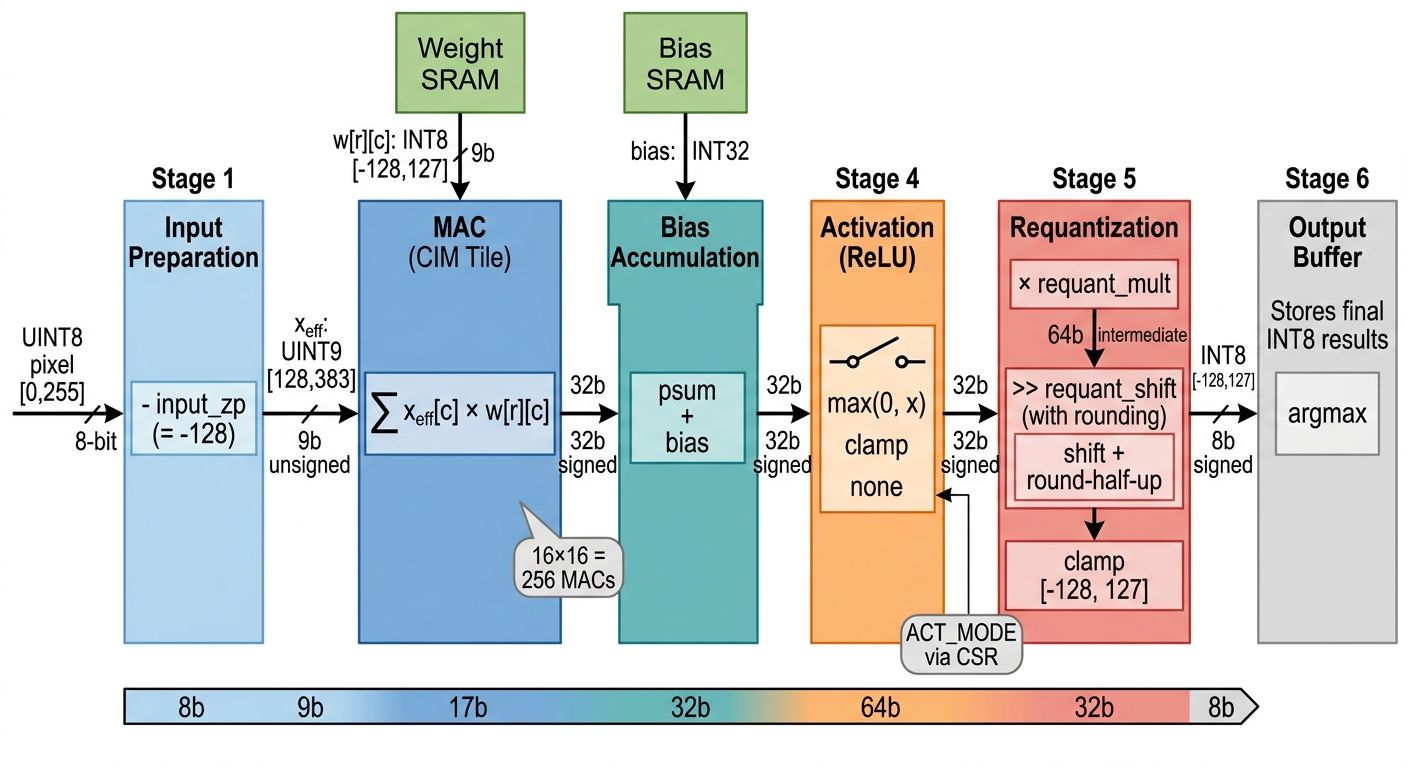
\includegraphics[width=0.95\textwidth]{figures/m5.png}
	\caption{INT8 CIM加速器完整数据通路：从输入准备到量化输出的6级流水}
	\label{fig:arch}
\end{figure}

系统由以下关键模块组成：
\begin{itemize}
	\item \textbf{cim\_accel\_core}：核心加速器引擎，包含17状态的FSM与7级流水线，负责计算调度与性能计数；
	\item \textbf{cim\_tile}：16×16 CIM原子计算单元，纯组合逻辑，实现256个INT8 MAC运算；
	\item \textbf{psum\_accum}：部分和累加器，带优先级清零机制；
	\item \textbf{weight\_sram}：16-bank权重SRAM，支持AXI DMA写入与tile-packed读取；
	\item \textbf{bias\_sram}：偏置SRAM，按输出神经元索引寻址；
	\item \textbf{input\_buffer}：输入缓冲，支持AXI写入与零点减法；
	\item \textbf{output\_buffer}：输出缓冲，含argmax逻辑；
	\item \textbf{cim\_axi\_lite\_slave}：AXI4-Lite接口，提供CSR配置与存储窗口访问。
\end{itemize}

所有可配置参数集中管理于\texttt{cim\_pkg.sv}包中，包括Tile尺寸（TILE\_ROWS=16, TILE\_COLS=16）、并行度（PAR\_OB）、数据位宽（INT8输入/权重、INT32偏置/累加器）、最大层维度（MAX\_IN\_DIM=784, MAX\_OUT\_DIM=128）、CSR地址映射与FSM状态编码。全局无魔法数字，所有RTL模块通过\texttt{import cim\_pkg::*}引用参数。

加速器的工作流程为：PS（或PicoRV32）通过AXI接口写入权重、偏置与输入数据，配置层参数（IN\_DIM, OUT\_DIM, N\_IB, N\_OB, requant\_mult, requant\_shift, act\_mode, input\_zp），然后触发start信号。核心引擎按output-block并行、input-block迭代的顺序完成MVM运算，每轮计算后进行偏置累加、激活与重量化，最终将INT8结果写入输出缓冲。完成后置位done信号并可触发IRQ。

\subsection{CIM Tile设计}

CIM Tile是本设计的原子计算单元，实现以下运算：

\begin{equation}
	\text{psum}[r] = \sum_{c=0}^{15} \text{x\_eff}[c] \times w[r][c], \quad r = 0, 1, \ldots, 15
\end{equation}

其中$\text{x\_eff}$为经过零点减法后的9位无符号有效输入，$w$为Signed-INT8权重，输出为32位有符号部分和。原始UINT8像素值$[0,255]$减去零点$\text{input\_zp}=-128$（即加上128），得到范围为$[128,383]$的9位无符号值。

Tile采用纯组合逻辑实现，通过generate构造16行×16列的乘加阵列（如图\ref{fig:cim_tile}所示）。每行独立计算一个输出神经元的部分和，列方向采用链式累加：

\begin{equation}
	\text{row\_acc}[c+1] = \text{row\_acc}[c] + \text{signed\_extend}(\text{x\_eff}[c]) \times w[r][c]
\end{equation}

每个Tile每个时钟周期产生$16 \times 16 = 256$个MAC运算的结果。采用纯组合设计的原因是将时序控制集中在核心引擎的FSM中，Tile本身作为"存储阵列做计算"的数字抽象。

\begin{figure}[H]
	\centering
	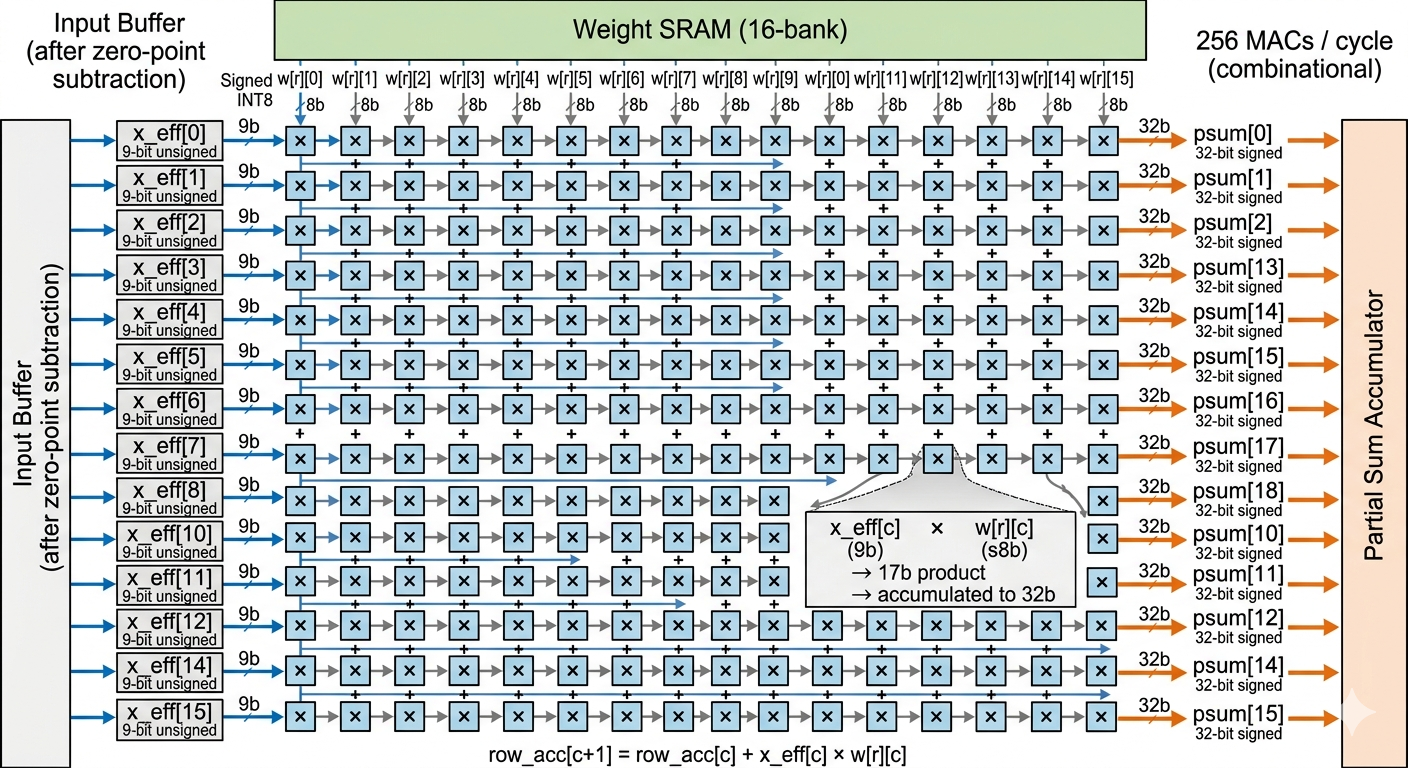
\includegraphics[width=0.75\textwidth]{figures/m3.png}
	\caption{16$\times$16 CIM Tile内部架构：输入广播、权重列与链式累加}
	\label{fig:cim_tile}
\end{figure}

\subsection{存储子系统}

\subsubsection{权重SRAM的BRAM推断问题与bank拆分方案}

权重SRAM的设计是本项目的关键工程挑战之一。初始设计中，weight SRAM为一整块2048位宽（$\text{TILE\_ROWS} \times \text{TILE\_COLS} \times 8 = 2048$位）的存储器。然而，Vivado对这种超宽memory推断BRAM本身就困难；更关键的是，如果用bit-select方式做32位chunk部分写入，Vivado会直接放弃BRAM推断，退化为纯寄存器，导致资源爆炸。

解决方案是将weight SRAM拆分为16个独立的bank（如图\ref{fig:weight_sram_bank}所示），每个bank仅$\text{ROW\_W} = \text{TILE\_COLS} \times \text{WEIGHT\_W} = 128$位宽，对应Tile的一行权重。16个bank通过generate实例化，每个bank独立推断为BRAM：

\begin{equation}
	\text{bank\_mem}[r][\text{tile\_idx}] = \{w[r][15], w[r][14], \ldots, w[r][0]\}, \quad r = 0, \ldots, 15
\end{equation}

写入侧，AXI slave使用staging register将4个32位AXI写入累积为完整的128位行数据，然后通过单周期whole-word写入送入对应bank。这确保了BRAM推断所需的"纯整字写入"条件。

\begin{figure}[H]
	\centering
	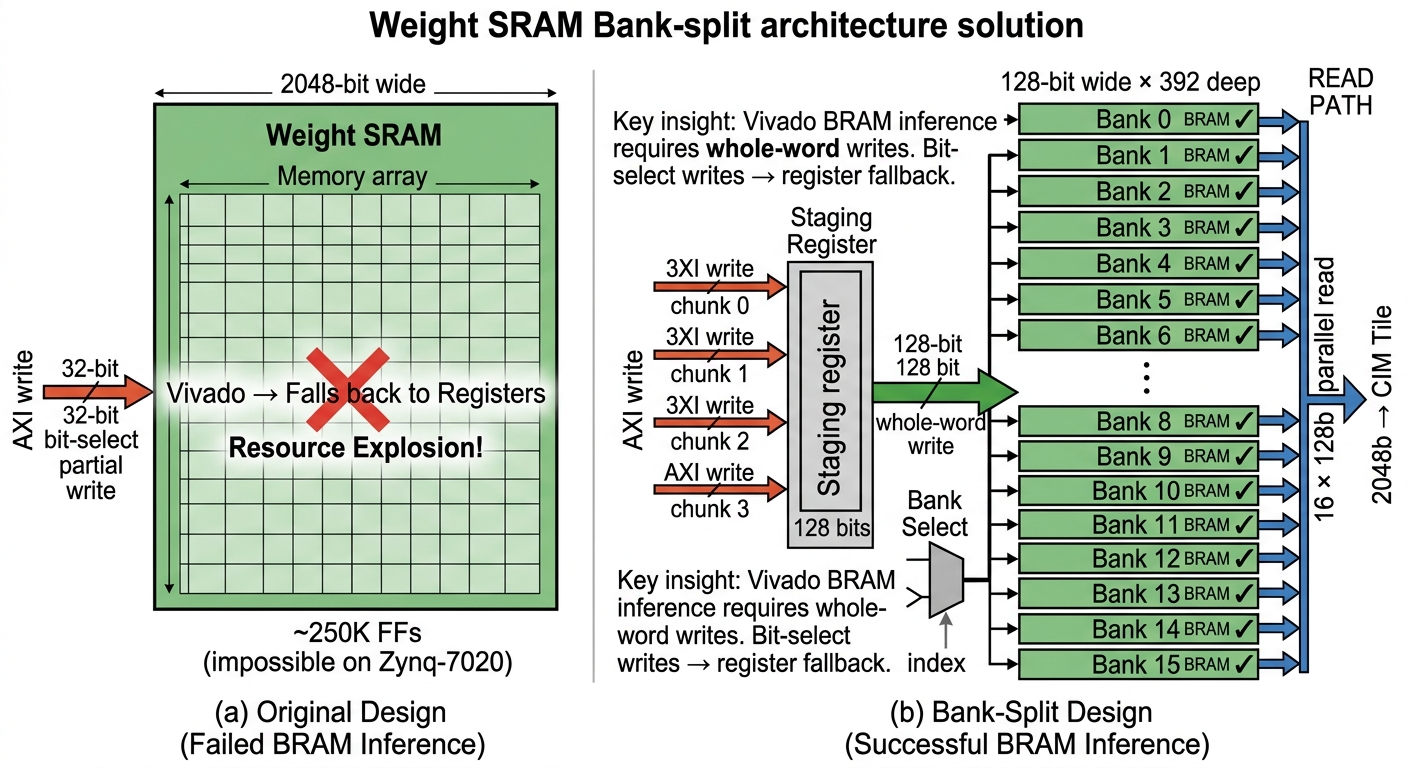
\includegraphics[width=0.85\textwidth]{figures/m4.png}
	\caption{权重SRAM的bank拆分方案：从BRAM推断失败到成功}
	\label{fig:weight_sram_bank}
\end{figure}

\begin{table}[H]
	\centering
	\caption{权重SRAM设计参数}
	\begin{tabular}{lcc}
		\toprule
		参数 & 值 & 说明 \\
		\midrule
		Bank数量 & 16 & 对应TILE\_ROWS \\
		Bank宽度 & 128 bits & TILE\_COLS $\times$ WEIGHT\_W \\
		Bank深度 & 392 & MAX\_N\_OB $\times$ MAX\_N\_IB = $8 \times 49$ \\
		总容量 & 100,352 bytes & $16 \times 128 \times 392 / 8$ \\
		写入接口 & 128-bit whole-word & 确保BRAM推断 \\
		读取延迟 & 1 cycle & registered read \\
		\bottomrule
	\end{tabular}
\end{table}

\subsubsection{偏置SRAM与输入缓冲}

偏置SRAM按输出神经元索引寻址，每个条目32位（INT32），深度为MAX\_OUT\_DIM=128。输入缓冲存储tile-packed的输入数据，每条目$\text{TILE\_COLS} \times \text{INPUT\_W} = 128$位，深度为MAX\_N\_IB=49。输入缓冲在读取时自动完成零点减法：

\begin{equation}
	\text{x\_eff}[c] = \text{input}[c] - \text{input\_zp}
\end{equation}

其中input\_zp通过CSR配置，默认为$-128$（相当于将UINT8像素值整体上移128，确保x\_eff为非负的9位无符号值，范围$[128,383]$）。

\subsection{量化与重定标}

本设计的量化流程遵循标准INT8整数推理规范（完整数据通路如图\ref{fig:arch}所示）\cite{6}，确保与软件golden model的bit-exact一致性。完整的量化链路为：

\begin{equation}
	\text{psum} = \sum_c \text{x\_eff}[c] \times w[r][c] + \text{bias}[r]
\end{equation}

\begin{equation}
	\text{prod} = \text{psum} \times \text{requant\_mult}
\end{equation}

\begin{equation}
	\text{shifted} = \left\lfloor \frac{\text{prod} + 2^{\text{requant\_shift}-1}}{2^{\text{requant\_shift}}} \right\rfloor
\end{equation}

\begin{equation}
	\text{output} = \text{clamp}(\text{shifted}, -128, 127)
\end{equation}

其中requant\_mult和requant\_shift为每层可配置的量化参数，通过CSR在运行时设置。重定标过程中使用64位中间乘积以避免溢出，移位时采用带舍入的算术右移（round-half-up），最后clamp到INT8范围$[-128, 127]$。

激活函数支持三种模式：无激活（ACT\_NONE）、ReLU（ACT\_RELU，将负值归零）、范围截断（ACT\_CLAMP）。模式通过CSR的ACT\_MODE寄存器配置。

\subsection{AXI4-Lite接口}

系统通过AXI4-Lite slave接口与外部控制器（PS ARM或PicoRV32）交互，采用14位地址空间（16KB），划分为以下区域：

\begin{table}[H]
	\centering
	\caption{CSR地址映射}
	\begin{tabular}{lcl}
		\toprule
		地址范围 & 偏移 & 功能 \\
		\midrule
		0x000--0x00C & & 控制/状态/IRQ寄存器 \\
		0x010--0x02C & & 层配置（IN\_DIM, OUT\_DIM, N\_IB, N\_OB, 量化参数） \\
		0x030--0x03C & & 性能计数器（cycle count, MAC count） \\
		0x040 & & argmax预测结果 \\
		0x044--0x04C & & 权重DMA控制（地址/数据/控制） \\
		0x100--0x2FF & & Logits回读窗口 \\
		0x1000--0x1FFF & & 输入缓冲写入窗口 \\
		0x2000--0x2FFF & & 偏置缓冲写入窗口 \\
		\bottomrule
	\end{tabular}
\end{table}

权重写入采用DMA式接口：软件设置CSR\_WDMA\_ADDR（tile索引）与CSR\_WDMA\_DATA（32位数据块），通过CSR\_WDMA\_CTRL的chunk\_idx字段指定当前写入的是128位行的第几个32位块。AXI slave内部使用staging register累积4个chunk后，生成一次128位whole-word写入到weight\_sram。

\subsection{7级流水线状态机}

核心引擎的FSM包含17个状态，其中计算数据通路划分为7级流水线，分为两个流水区域：

\textbf{计算流水线}（每个input-block迭代）：
\begin{enumerate}
	\item \textbf{ST\_FETCH / ST\_WAIT\_SRAM}：发出BRAM读地址，等待权重SRAM输出（1 cycle latency）；
	\item \textbf{ST\_XEFF\_REG}：输入BRAM输出就绪 + 零点减法 → 锁存x\_eff\_reg。关键路径：BRAM $T_{co}$ + 32位减法 + clamp（约10 ns）；
	\item \textbf{ST\_MAC}：cim\_tile计算 x\_eff\_reg $\times$ w\_tile\_reg → 锁存tile\_psum\_reg。关键路径：16元素MAC链（约10 ns）；
	\item \textbf{ST\_COMPUTE}：psum\_accum += tile\_psum\_reg（寄存器加法）。关键路径：32位加法（约4 ns）。
\end{enumerate}

\textbf{输出流水线}（每个output neuron，所有IB迭代完成后）：
\begin{enumerate}
	\setcounter{enumi}{4}
	\item \textbf{ST\_BIAS\_ADD → ST\_ACTIVATE}：加偏置 → ReLU激活；
	\item \textbf{ST\_STORE}：64位乘法（psum $\times$ requant\_mult）→ 锁存prod\_r；
	\item \textbf{ST\_SHIFT\_CLAMP → ST\_WRITE\_OBUF}：移位 + 舍入 + clamp → 写输出缓冲。
\end{enumerate}

将原本的26ns组合路径拆分为多级流水后，每级关键路径控制在约10ns以内。代价是每个IB迭代增加2个额外周期（XEFF\_REG + MAC），对于FC1层（49个IB迭代），计算周期从约392增加到约539。这一权衡使得设计可以在更高频率下工作。

\begin{figure}[H]
	\centering
	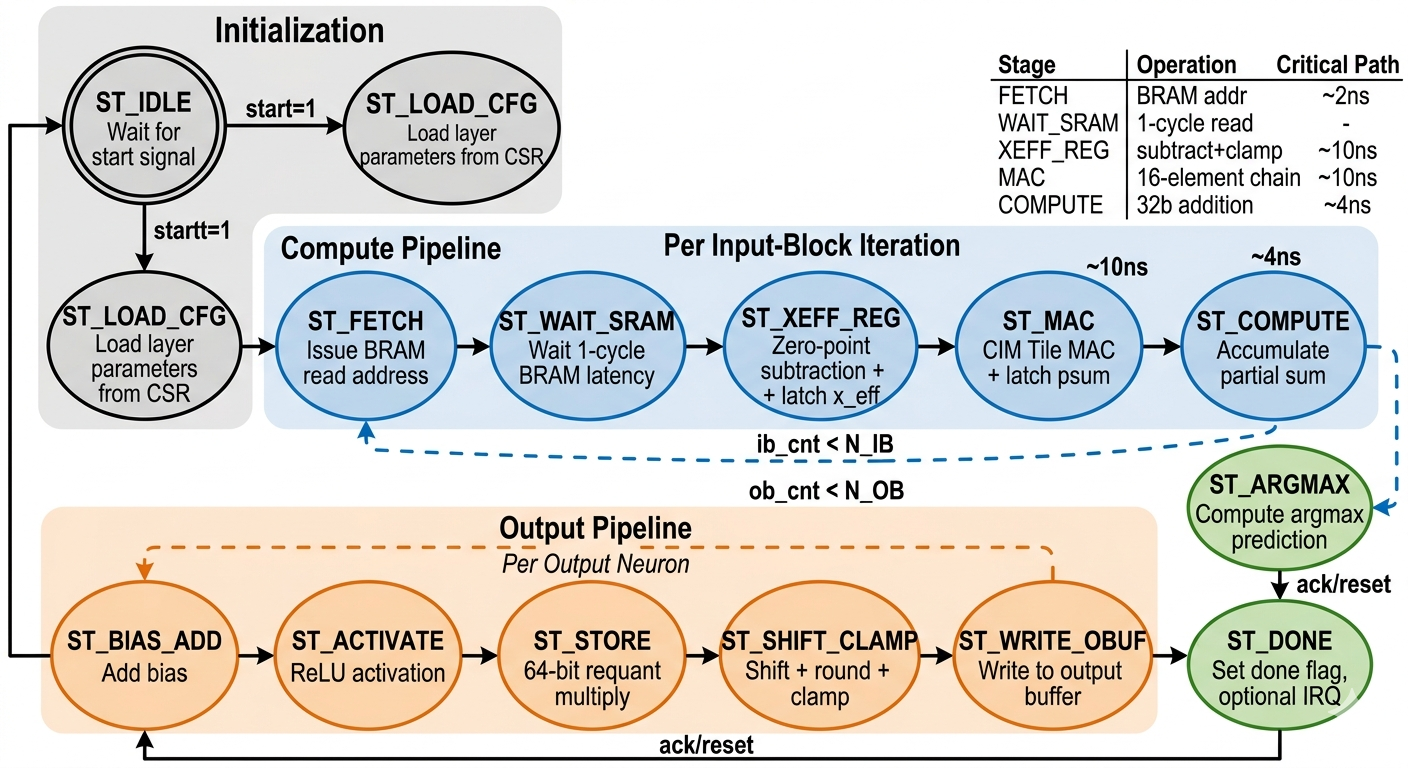
\includegraphics[width=0.95\textwidth]{figures/m6.png}
	\caption{17状态FSM状态转移图：初始化、计算流水线与输出流水线}
	\label{fig:fsm_states}
\end{figure}

图\ref{fig:fsm_states}展示了完整的FSM状态转移关系。计算流水线中ST\_FETCH到ST\_COMPUTE构成内循环（按input-block迭代），输出流水线中ST\_BIAS\_ADD到ST\_WRITE\_OBUF构成外循环（按output neuron迭代）。

\begin{figure}[H]
	\centering
	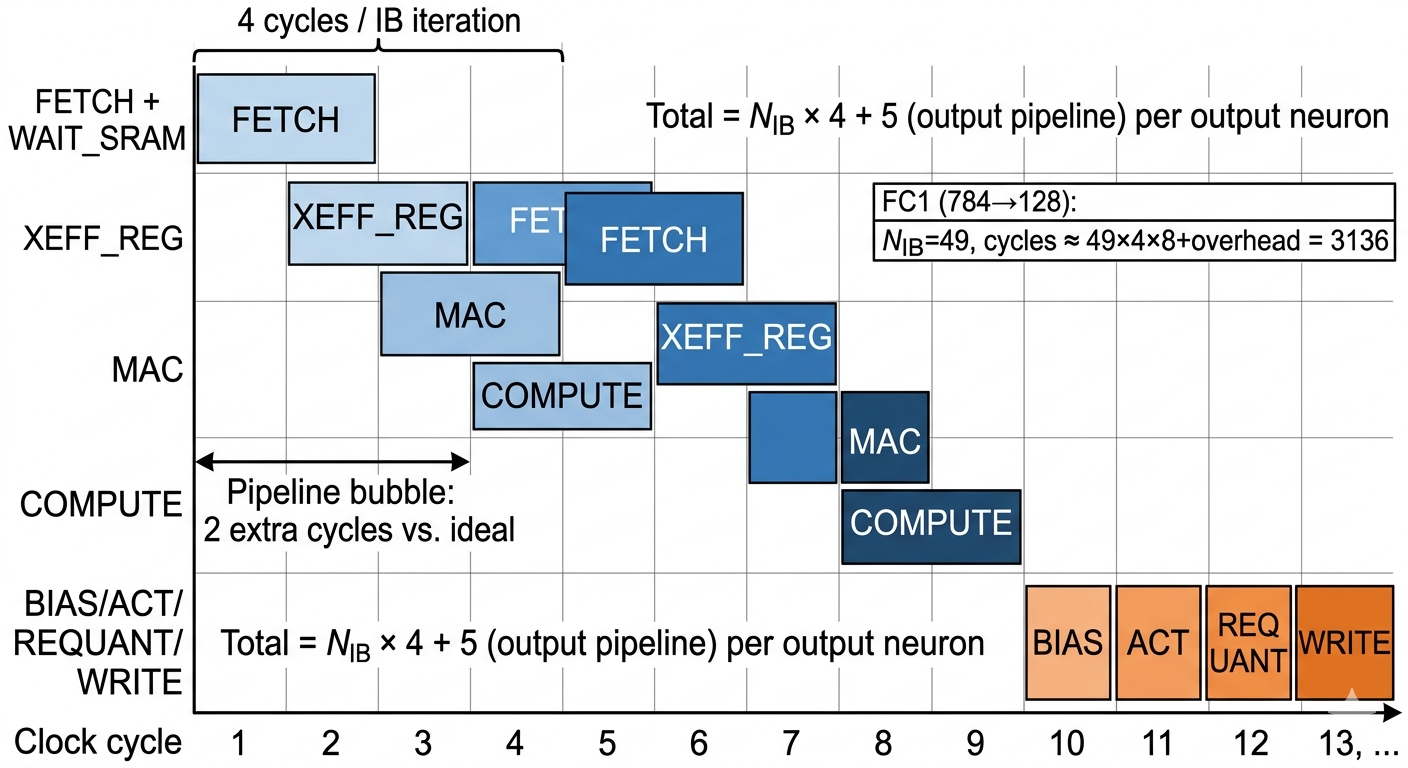
\includegraphics[width=0.9\textwidth]{figures/m7.png}
	\caption{流水线时序图：多个input-block迭代的重叠执行}
	\label{fig:pipeline_timing}
\end{figure}

图\ref{fig:pipeline_timing}展示了连续input-block迭代的流水线执行时序。每个IB迭代约需4个时钟周期，相邻迭代之间存在2个周期的流水线气泡。

% ====================================================================
\section{PicoRV32 RISC-V软核集成}
% ====================================================================

\subsection{设计动机}

Step 1-3中的CIM加速器由ARM PS通过Python/MMIO控制。然而，项目任务指导书要求实现软核设计，因此不应该直接使用ARM PS，而需要在PL侧实现自主控制能力。本设计选择集成PicoRV32开源RISC-V软核（YosysHQ，MIT License），其优势包括：

\begin{itemize}
	\item 单文件实现（\texttt{picorv32.v}），RV32IM指令集；
	\item 资源开销低：约1500 LUT；
	\item 成熟的native memory interface，适合直接桥接到CIM CSR。
\end{itemize}

最终目标是让CIM加速器在纯PL中自主运行推理，不依赖PS控制。

\subsection{系统架构}

PicoRV32集成后的系统架构如图\ref{fig:rv32_arch}所示。

\begin{figure}[H]
	\centering
	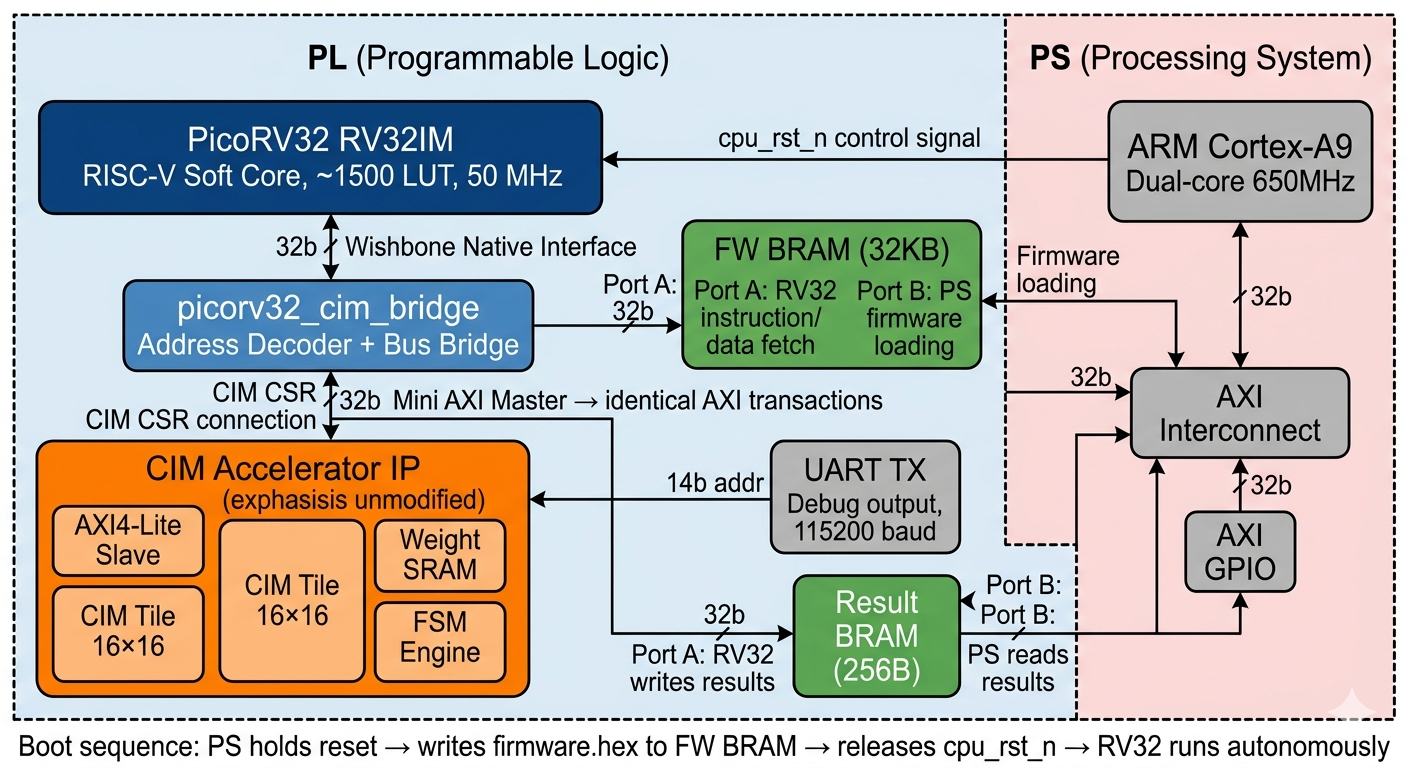
\includegraphics[width=0.95\textwidth]{figures/m8.png}
	\caption{PicoRV32 + CIM SoC系统架构：PL侧RISC-V软核与CIM IP集成}
	\label{fig:rv32_arch}
\end{figure}

设计要点包括：

（1）\textbf{CIM IP不做修改}：PicoRV32通过mini AXI master发送与ARM完全相同的AXI事务，CIM IP的AXI slave接口无需任何改动，确保了与Step 2硬件的完全兼容。

（2）\textbf{双端口FW BRAM}：固件通过PS侧AXI写入FW BRAM port B，而不是烧写到bitstream中。这使得每次更换测试图片无需重新生成bitstream，只需重新加载firmware.hex。FW BRAM容量32KB，足以容纳784→16→10小型MLP模型的权重数据与C固件代码（约14.5KB）。

（3）\textbf{Result BRAM}：PicoRV32将推理结果（预测类别、logits、magic标记）写入Result BRAM，PS通过AXI读取结果。这避免了PL侧UART与PS侧USB的连接性问题。

（4）\textbf{CPU复位控制}：PS通过AXI GPIO控制cpu\_rst\_n信号，实现"hold → write firmware → release"的操作流程。

\subsection{Bus Bridge与地址映射}

\texttt{picorv32\_cim\_bridge}模块将PicoRV32的native memory interface桥接到各外设，地址映射如图\ref{fig:rv32_addr_map}和下表所示：

\begin{table}[H]
	\centering
	\caption{PicoRV32地址映射}
	\begin{tabular}{lcl}
		\toprule
		地址范围 & 大小 & 设备 \\
		\midrule
		0x0000\_0000 -- 0x0000\_7FFF & 32KB & FW BRAM (port A) \\
		0x4000\_0000 -- 0x4000\_3FFF & 16KB & CIM CSR / 存储窗口 \\
		0x8000\_0000 & 4B & UART TX数据寄存器 \\
		0x8000\_0004 & 4B & UART TX状态寄存器 \\
		0xC000\_0000 -- 0xC000\_00FF & 256B & Result BRAM (port A) \\
		\bottomrule
	\end{tabular}
\end{table}

Bridge根据地址高位进行译码，对CIM CSR区域的访问转换为AXI读写事务。PicoRV32访问CIM的流程与ARM通过MMIO访问完全等价，固件中的CSR读写函数直接对应AXI事务。

\begin{figure}[H]
	\centering
	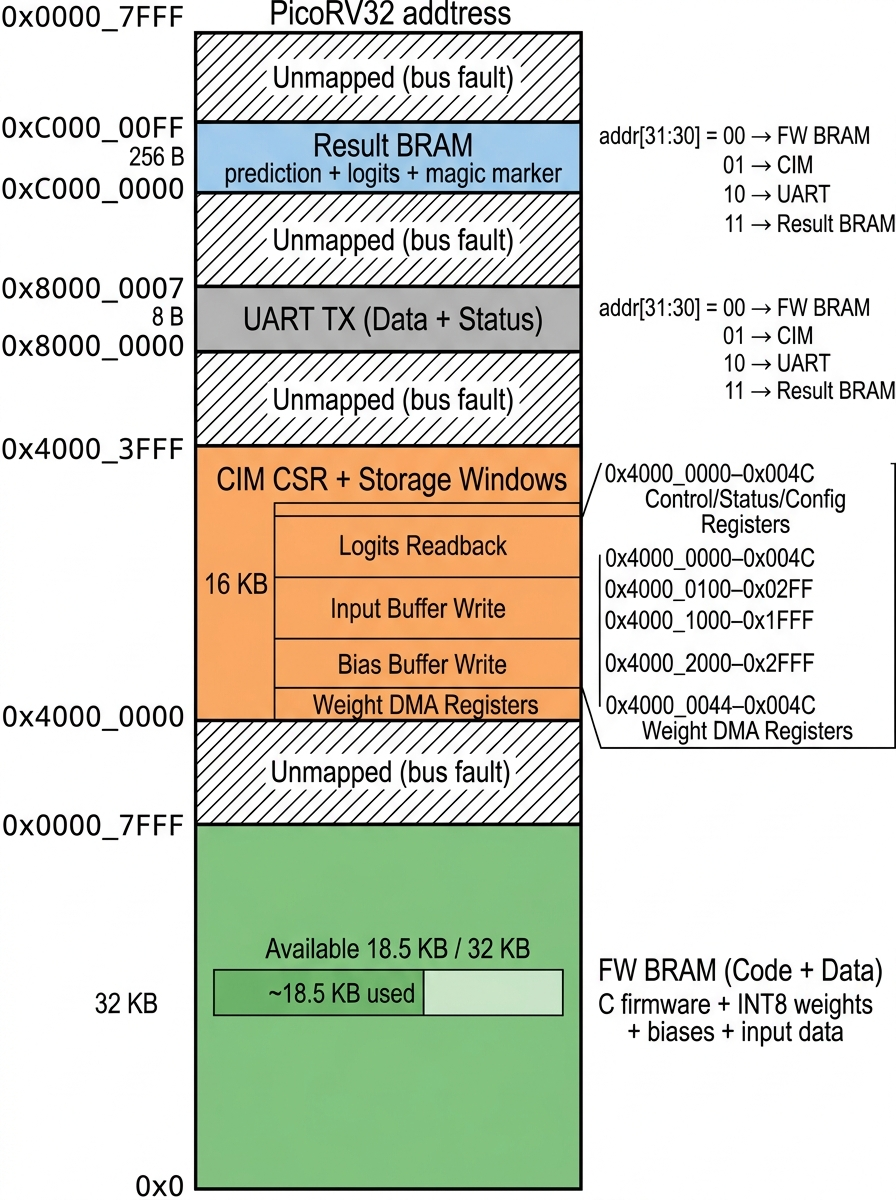
\includegraphics[width=0.5\textwidth]{figures/m9.png}
	\caption{PicoRV32地址空间映射与Bridge译码逻辑}
	\label{fig:rv32_addr_map}
\end{figure}

\subsection{模型规模约束}

由于PicoRV32额外占用LUT资源，且固件需要放入32KB FW BRAM，模型规模受到限制。FW BRAM中需要存储：C固件代码、权重数据（INT8打包）、偏置数据（INT32）与输入数据。对于784→16→10的小型MLP模型，数据量约为：

\begin{equation}
	784 \times 16 \times 1 + 16 \times 10 \times 1 + (16 + 10) \times 4 + 784 \times 1 \approx 14.5\text{KB}
\end{equation}

加上C固件代码约4KB，总计约18.5KB，可以放入32KB BRAM中。该模型在MNIST测试集上INT8量化推理准确率超过90\%。

% ====================================================================
\section{FPGA验证与性能评估}
% ====================================================================

\subsection{验证方法学}

本项目建立了"Python golden model → VCS仿真 → PYNQ上板"三层一致的验证方法学（如图\ref{fig:verification_flow}所示）：

\textbf{第一层：Python bit-accurate参考模型}。\texttt{golden\_model.py}以纯整数算术实现与硬件完全相同的计算流程（零点减法、MVM、偏置累加、ReLU、重量化），输出hex格式测试向量供RTL仿真和板级验证使用。

\textbf{第二层：VCS RTL仿真}。采用"单元级→阵列级→系统级"分层验证策略：
\begin{itemize}
	\item \textbf{tb\_cim\_tile}：CIM Tile单元测试，103个随机向量，验证MAC运算正确性；
	\item \textbf{tb\_cim\_accel\_core}：系统级MVM测试，覆盖随机向量与边界用例（全零、全$-128$、最大维度等）；
	\item \textbf{tb\_mnist\_e2e}：MNIST端到端测试，784→128→10两层MLP，与golden model逐元素对比。
\end{itemize}

通过\texttt{run\_regression.sh}脚本一键运行全部测试并汇总PASS/FAIL结果。

\textbf{第三层：PYNQ-Z2上板验证}。将bitstream与hwh文件部署到PYNQ板，通过Jupyter Notebook运行Python驱动程序（\texttt{cim\_driver.py}的\texttt{CIMModel}类），加载真实MNIST手写数字图片，逐层执行推理并与golden model对比。

\begin{figure}[H]
	\centering
	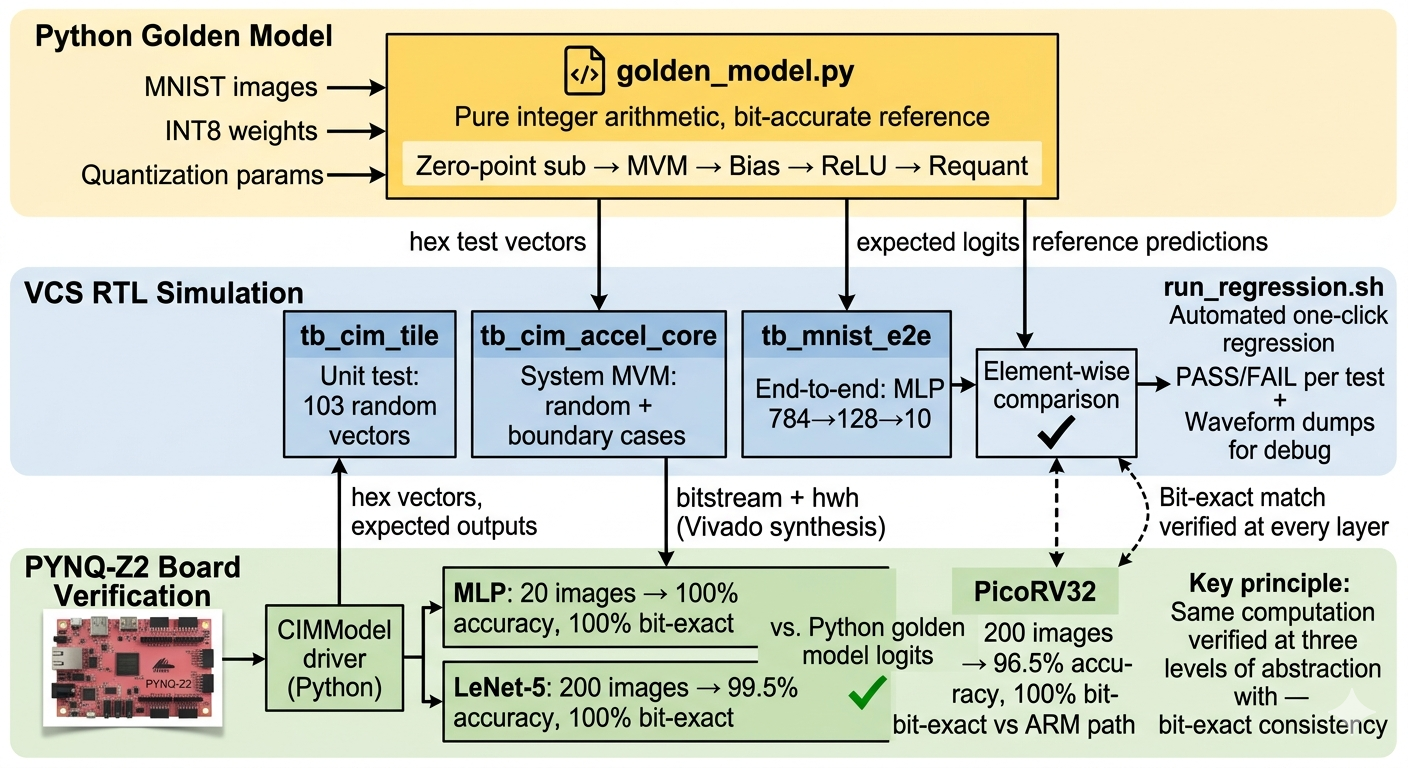
\includegraphics[width=0.95\textwidth]{figures/m10.png}
	\caption{三层验证方法学流程：Python Golden Model → VCS RTL仿真 → PYNQ板级验证}
	\label{fig:verification_flow}
\end{figure}

\subsection{PYNQ-Z2综合结果}

设计在Vivado 2024.2中针对Zynq-7020（xc7z020clg400-1）进行综合与实现。以下为ARM控制模式（不含PicoRV32）的综合结果，表\ref{tab:util_arm}列出了各类资源的使用量与占用率。

\begin{table}[H]
	\centering
	\caption{CIM SoC资源占用（ARM控制模式，PAR\_OB=1，PYNQ-Z2）}
	\begin{tabular}{lccccc}
		\toprule
		资源类型 & 使用量 & 可用量 & 占用率 \\
		\midrule
		Slice LUT & 11,087 & 53,200 & 20.84\% \\
		\quad LUT as Logic & 11,027 & 53,200 & 20.73\% \\
		\quad LUT as Memory & 60 & 17,400 & 0.34\% \\
		Slice Register (FF) & 5,385 & 106,400 & 5.06\% \\
		Block RAM (36Kb) & 34 & 140 & 24.29\% \\
		Block RAM (18Kb) & 2 & 280 & 0.71\% \\
		DSP48E1 & 220 & 220 & 100.00\% \\
		\bottomrule
	\end{tabular}
	\label{tab:util_arm}
\end{table}

图\ref{fig:resource_util}以柱状图形式对比了两种控制模式的资源占用，图\ref{fig:floorplan}展示了Vivado布局布线后芯片上各模块的物理分布。DSP占用率达到100\%是因为PAR\_OB=1时，CIM Tile的16×16=256个乘法器中的大部分映射到了DSP48E1。Zynq-7020共有220个DSP48，恰好被完全利用。如果需要降低DSP占用，可以通过Vivado综合属性将部分乘法器映射到LUT。

时序方面，如表\ref{tab:timing_arm}所示，时钟约束为60 MHz（16.7 ns周期），布局布线后WNS（最差负裕量）为$-0.086$ns，存在轻微时序违例（3个failing endpoints），但实际上板测试中功能完全正确。关键路径位于CIM Tile的MAC链。

\begin{table}[H]
	\centering
	\caption{时序与功耗（ARM控制模式）}
	\begin{tabular}{lc}
		\toprule
		指标 & 值 \\
		\midrule
		目标时钟频率 & 60 MHz \\
		时钟约束 & 16.7 ns \\
		WNS & $-0.086$ ns \\
		总功耗 & 1.954 W \\
		\quad PS7 & 1.520 W \\
		\quad CIM IP & 0.284 W \\
		\quad AXI Peripheral & 0.003 W \\
		\quad 静态功耗 & 0.147 W \\
		\bottomrule
	\end{tabular}
	\label{tab:timing_arm}
\end{table}

CIM IP本身动态功耗仅0.284 W，而PS7（ARM Cortex-A9双核 + DDR控制器）消耗1.520 W，占总功耗的主要部分。

\begin{figure}[H]
	\centering
	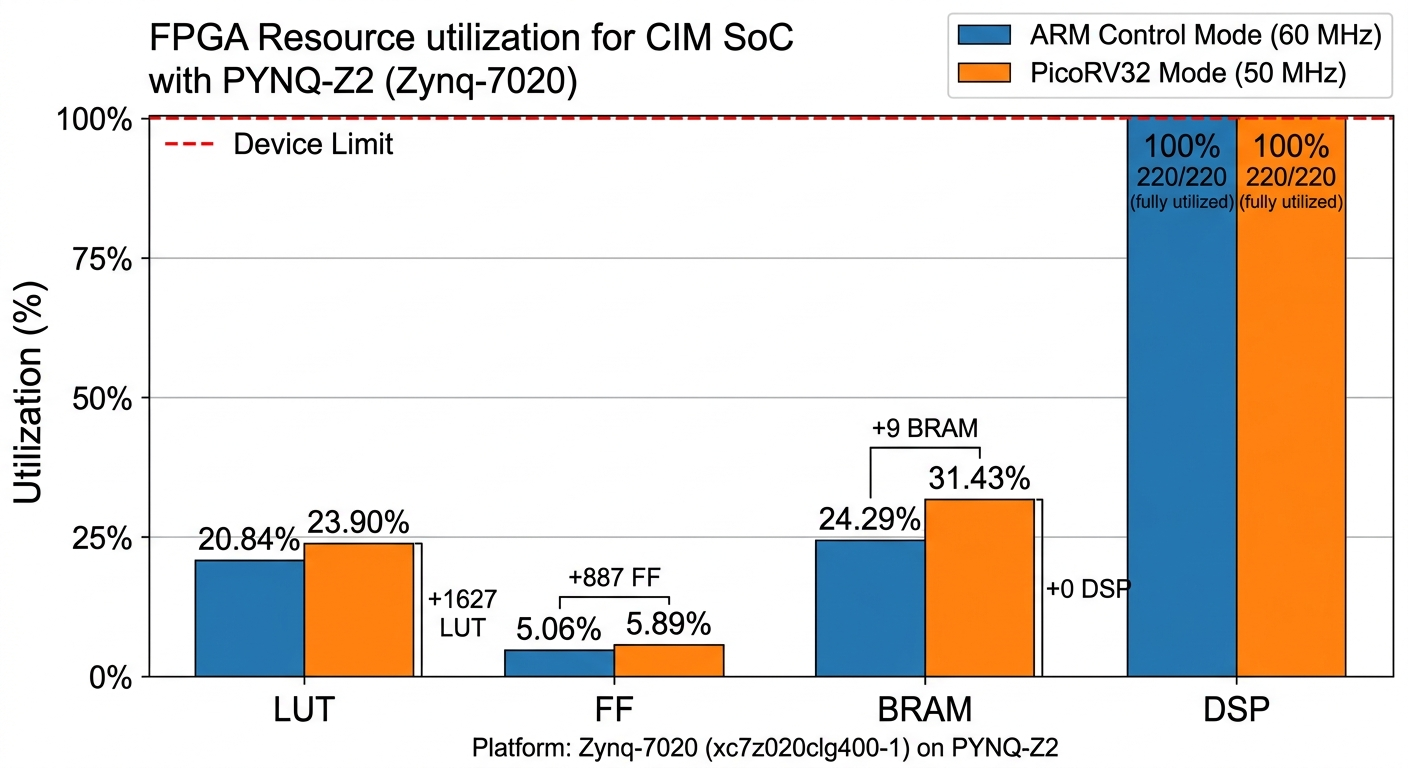
\includegraphics[width=0.85\textwidth]{figures/m11.png}
	\caption{FPGA资源占用率对比：ARM控制模式与PicoRV32模式}
	\label{fig:resource_util}
\end{figure}

\begin{figure}[H]
	\centering
	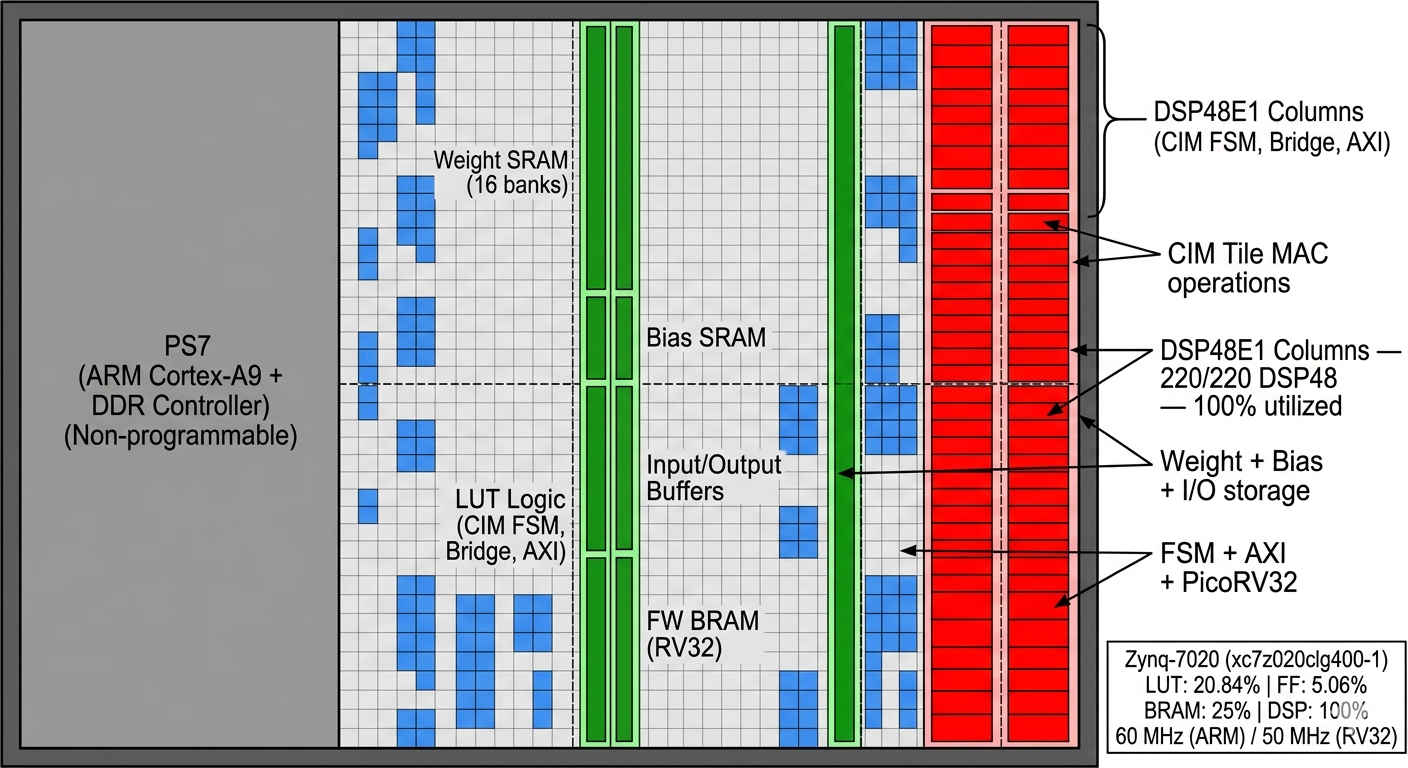
\includegraphics[width=0.85\textwidth]{figures/m15.png}
	\caption{Vivado布局布线结果：Zynq-7020芯片上CIM SoC各模块物理分布}
	\label{fig:floorplan}
\end{figure}

\subsection{MLP网络推理验证}

在ARM控制模式下，使用784→128→10两层MLP网络（INT8量化，量化后MNIST测试集准确率约93\%）进行上板验证。表\ref{tab:mlp_perf}给出了各层的推理周期数与MAC操作数。

\begin{table}[H]
	\centering
	\caption{MLP推理性能（PAR\_OB=1，60 MHz）}
	\begin{tabular}{lccc}
		\toprule
		层 & 维度 & 周期数 & MAC操作数 \\
		\midrule
		FC1 & 784→128 & 3,136 & 100,352 \\
		FC2 & 128→10 & 146 & 2,048 \\
		\midrule
		总计 & & 3,282 & 102,400 \\
		\bottomrule
	\end{tabular}
	\label{tab:mlp_perf}
\end{table}

单幅推理总延迟为：
\begin{equation}
	T_{\text{MLP}} = \frac{3282}{60 \times 10^6} = 54.7\,\mu\mathrm{s}
\end{equation}

在20张真实MNIST手写数字测试中，硬件输出与Python golden model的FC1全部128维输出、FC2全部10维logits逐元素完全一致（bit-exact），分类准确率100\%（20/20）。

\subsection{LeNet-5 CNN推理验证}

LeNet-5是一个包含2个卷积层、2个最大池化层和3个全连接层的经典CNN。由于CIM硬件本身只支持MVM运算，卷积层通过软件侧im2col变换转化为矩阵乘法后喂给硬件引擎。im2col将卷积的滑窗操作展开为一个大矩阵，使得$\text{col\_len} = C_{in} \times K \times K$作为MVM的输入维度。表\ref{tab:lenet5_perf}列出了各层的推理周期数。

\begin{table}[H]
	\centering
	\caption{LeNet-5各层推理周期数（PAR\_OB=1，60 MHz）}
	\begin{tabular}{lcccc}
		\toprule
		层 & 类型 & 维度 & 平均周期数 \\
		\midrule
		conv1 & Conv 5×5 & 1×28×28→6×24×24 & 63,360 \\
		conv2 & Conv 5×5 & 6×12×12→16×8×8 & 10,112 \\
		fc3 & FC & 400→120 & 1,552 \\
		fc4 & FC & 120→84 & 876 \\
		fc5 & FC & 84→10 & 134 \\
		\midrule
		总计 & & & 76,034 \\
		\bottomrule
	\end{tabular}
	\label{tab:lenet5_perf}
\end{table}

单幅推理总延迟为：
\begin{equation}
	T_{\text{LeNet5}} = \frac{76034}{60 \times 10^6} = 1.267 \text{ ms}
\end{equation}

在200张真实MNIST手写数字测试中：
\begin{itemize}
	\item 硬件分类准确率（vs 标签）：99.5\%（199/200）
	\item 与Python golden model的bit-exact一致率：100.0\%（200/200）
	\item 计算错误数：0
\end{itemize}

图\ref{fig:mnist_results}展示了部分分类结果。200张图片中唯一的"错误"分类（img\_0018，标签3预测为8）与Python golden model的预测完全一致，说明这是INT8量化精度损失导致的，而非硬件计算错误。全部200张图片的全部层输出均与Python参考模型bit-exact一致，验证了硬件实现的正确性。

\begin{figure}[H]
	\centering
	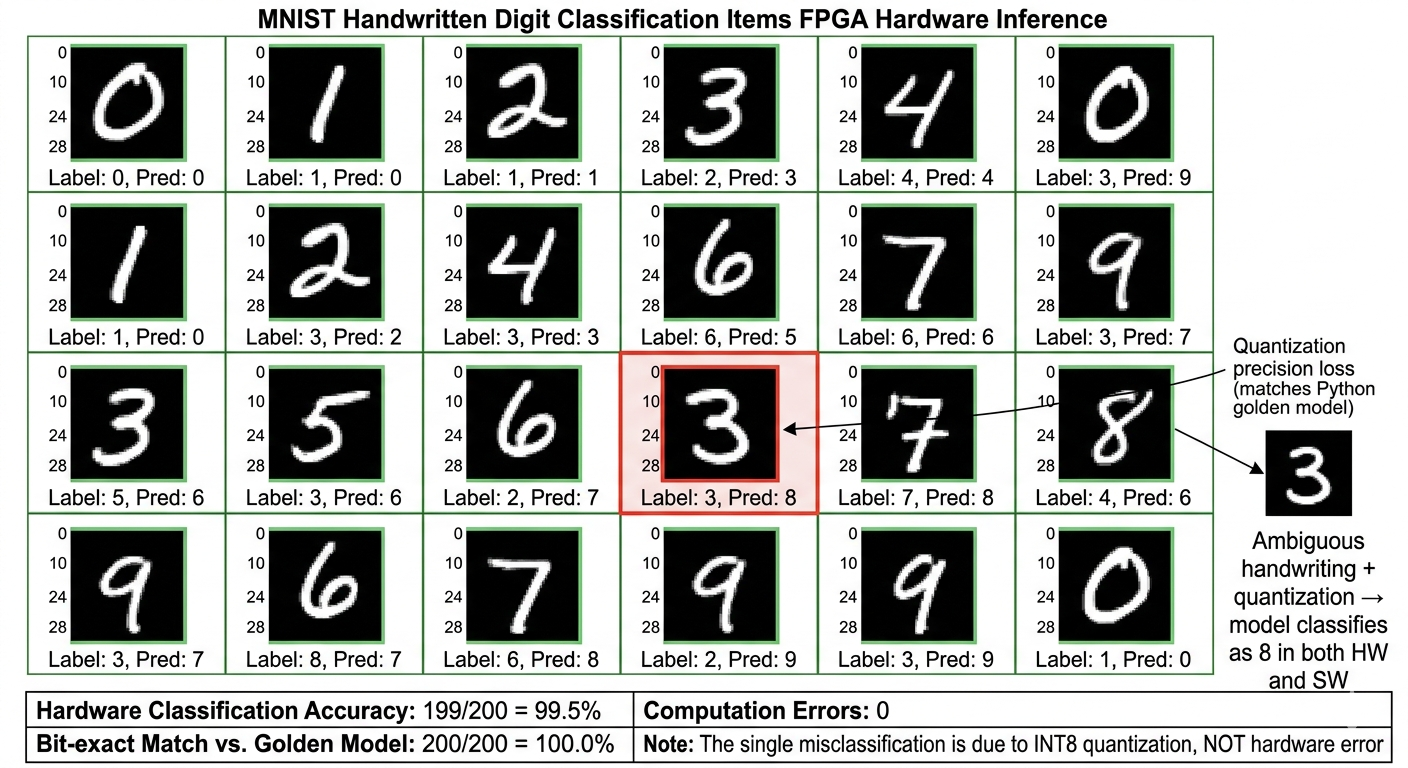
\includegraphics[width=0.85\textwidth]{figures/m12.png}
	\caption{LeNet-5硬件推理MNIST分类结果：200张手写数字图片}
	\label{fig:mnist_results}
\end{figure}

启用下一小节所述的SQ-mapping软件映射优化（§\ref{sec:sqmapping}）后，实际上板运行200张LeNet-5推理的总wall time为340.1秒（1.700秒/张），其中绝大部分时间消耗在Python驱动的MMIO数据搬运上，硬件计算本身仅占1.267 ms/张。

\subsection{SQ-mapping 软件映射优化}
\label{sec:sqmapping}

在LeNet-5这类小卷积核网络中，直接把im2col得到的每个输出像素逐一送入MVM引擎会严重浪费CIM阵列的利用率。以Conv1层（$1\times5\times5\to6$）为例，单次MVM的有效输入维度仅为$\text{col\_len} = C_{in}\times K_h\times K_w = 25$，而硬件支持的$\text{MAX\_IN\_DIM}=784$，利用率不足$25/784\approx 3.2\%$；同时单次MVM产生$C_{out}=6$个输出神经元，而硬件支持的$\text{MAX\_OUT\_DIM}=128$，输出侧利用率同样极低。这种"瘦长矩阵挤在大阵列里"的映射方式使得每次硬件调用的MMIO建立/搬运开销被完全暴露，无法被有效均摊。

借鉴师兄\texttt{cim\_wzy}项目\texttt{SQ\_MAPPING}思想，本文在\texttt{cim\_driver.py::CIMModel}中实现了一种\textbf{块对角权重打包}的软件映射优化：当$\text{col\_len}\times C_{out}$远小于硬件容量时，把$k_{\text{pack}}$个输出像素的im2col列与权重一起打包到同一次MVM调用中。具体来说，原始权重矩阵$W\in\mathbb{Z}^{C_{out}\times \text{col\_len}}$沿对角线复制$k_{\text{pack}}$份构造块对角矩阵：

\begin{equation}
	W_{\text{packed}} = \begin{bmatrix}
		W & & & \\
		& W & & \\
		& & \ddots & \\
		& & & W
	\end{bmatrix} \in \mathbb{Z}^{(k_{\text{pack}}\cdot C_{out})\times (k_{\text{pack}}\cdot \text{col\_len})}
\end{equation}

输入侧同时将$k_{\text{pack}}$个输出像素对应的im2col列串联成长向量。一次硬件调用即可同时得到$k_{\text{pack}}\cdot C_{out}$个输出神经元，再按$C_{out}$拆回$k_{\text{pack}}$组像素结果。打包因子由硬件维度上限决定：

\begin{equation}
	k_{\text{pack}} = \min\!\left(\left\lfloor\frac{\text{MAX\_IN\_DIM}}{\text{col\_len}}\right\rfloor,\ \left\lfloor\frac{\text{MAX\_OUT\_DIM}}{C_{out}}\right\rfloor\right)
\end{equation}

表\ref{tab:sqmapping}给出了LeNet-5两个卷积层的打包结果。

\begin{table}[H]
	\centering
	\caption{LeNet-5卷积层SQ-mapping打包前后对比}
	\label{tab:sqmapping}
	\small
	\begin{tabular}{lcccccc}
		\toprule
		层 & $\text{col\_len}$ & $C_{out}$ & $k_{\text{pack}}$ & 原始MVM次数 & 打包后MVM次数 & 理论加速比 \\
		\midrule
		Conv1 & 25 & 6 & 21 & 576 & 28 & $\approx 20.6\times$ \\
		Conv2 & 150 & 16 & 5 & 64 & 13 & $\approx 4.9\times$ \\
		\bottomrule
	\end{tabular}
\end{table}

该优化不需要修改任何RTL。正确性方面，启用SQ-mapping后逐层bit-exact验证全部通过（200张图全部层输出与Python golden model一致），分类准确率仍为99.5\%（199/200），与未打包时完全相同。

从端到端墙钟时间来看（表\ref{tab:sqmapping_walltime}），SQ-mapping将LeNet-5的每张推理时间从3.54秒降低到1.625秒，整体加速约\textbf{2.18倍}。加速比小于理论值（$\approx 20\times$）的原因是：打包只减少了卷积层的MVM调用次数，而全连接层（FC3--FC5）和MaxPool层的时间不受影响；加之每次MVM调用中$k_{\text{pack}}\times\text{col\_len}$更长，硬件周期数本身也略有增加。即便如此，2.18倍的端到端加速完全来自软件侧映射优化，是本工作对SQ-mapping思想在FPGA异构验证平台上的一次直接验证。

\begin{table}[H]
	\centering
	\caption{LeNet-5启用SQ-mapping前后的200张图片端到端墙钟时间}
	\label{tab:sqmapping_walltime}
	\begin{tabular}{lccc}
		\toprule
		配置 & 总wall time（s） & 单张平均（ms） & 准确率 \\
		\midrule
		逐像素调用（baseline） & 708.3 & 3,541.5 & 99.5\% \\
		SQ-mapping打包 & 340.1 & 1,700.4 & 99.5\% \\
		\midrule
		相对加速比 & \multicolumn{3}{c}{\textbf{2.08}$\times$} \\
		\bottomrule
	\end{tabular}
\end{table}

\subsection{加速比分析}

为量化CIM硬件加速效果，需要将硬件推理时间与纯软件基线进行对比。

\subsubsection{理论分析}

CIM硬件的核心优势在于利用存储阵列的并行性实现高通量MAC运算。以FC1层（784→128）为例：

\begin{itemize}
	\item 总MAC操作数：$784 \times 128 = 100,352$
	\item 硬件周期数：3,136
	\item 每周期有效MAC数：$100352 / 3136 = 32$ MACs/cycle
	\item 吞吐率（60 MHz）：$32 \times 60 \times 10^6 = 1.92 \text{ GMACs/s}$
\end{itemize}

而ARM Cortex-A9（Zynq-7020 PS，双核650 MHz）执行INT8矩阵乘法时，即使利用NEON SIMD指令，单核每周期最多执行8个INT8 MAC（128位SIMD寄存器 / 16位乘积），理论峰值吞吐率为$8 \times 650 \times 10^6 = 5.2 \text{ GMACs/s}$。但这一峰值假设了完美的数据复用与零延迟访存，实际效率受限于cache miss、指令开销与数据搬运，对于784×128这种中等规模矩阵，实际吞吐率通常远低于峰值。

\subsubsection{硬件推理时间}

根据性能计数器的实测数据，表\ref{tab:hw_latency}汇总了两个网络的硬件推理延迟：

\begin{table}[H]
	\centering
	\caption{CIM硬件推理延迟}
	\begin{tabular}{lccc}
		\toprule
		网络 & 总周期数 & 频率 & 推理延迟 \\
		\midrule
		MLP (784→128→10) & 3,282 & 60 MHz & 54.7 $\mu$s \\
		LeNet-5 (7层) & 76,034 & 60 MHz & 1,267 $\mu$s \\
		\bottomrule
	\end{tabular}
	\label{tab:hw_latency}
\end{table}

\subsubsection{端到端延迟拆解与瓶颈分析}
\label{sec:profiler}

为定位端到端延迟的真正瓶颈，本文在\texttt{cim\_driver.py::CIMModel.predict()}中插入细粒度profiler，将每一层的延迟拆分为四段：

\begin{itemize}
	\item \textbf{setup}：Python侧构造打包权重/bias矩阵、调用\texttt{weight\_to\_chunks}/\texttt{bias\_to\_u32}的时间；
	\item \textbf{load\_x}：通过AXI4-Lite逐字写入input\_buffer与weight\_sram的时间；
	\item \textbf{compute}：硬件性能计数器测得的纯MVM运算周期数除以时钟频率；
	\item \textbf{read}：从output\_buffer逐字读回结果的时间。
\end{itemize}

表\ref{tab:profiler}给出了LeNet-5单张图片在启用profiler模式下的各层延迟分布。

\begin{table}[H]
	\centering
	\caption{LeNet-5单张推理的逐层延迟拆解（PYNQ-Z2, 60 MHz, profiler模式）}
	\label{tab:profiler}
	\small
	\begin{tabular}{lrrrrr}
		\toprule
		层 & setup (ms) & load\_x (ms) & compute (ms) & read (ms) & total (ms) \\
		\midrule
		Conv1 (1$\to$6, 5$\times$5) & 315.8 & 332.9 & 4.6 & 194.2 & 892.9 \\
		MaxPool 2$\times$2 & -- & -- & -- & -- & 53.5 \\
		Conv2 (6$\to$16, 5$\times$5) & 283.0 & 219.0 & 1.9 & 56.5 & 569.5 \\
		MaxPool 2$\times$2 & -- & -- & -- & -- & 15.9 \\
		FC3 (256$\to$120) & 155.9 & 6.0 & 0.1 & 6.5 & 169.1 \\
		FC4 (120$\to$84) & 58.1 & 2.9 & 0.1 & 4.7 & 66.2 \\
		FC5 (84$\to$10) & 7.7 & 2.2 & 0.1 & 0.6 & 10.9 \\
		\midrule
		\textbf{合计} & \textbf{820.5} & \textbf{563.0} & \textbf{6.8} & \textbf{262.5} & \textbf{1778.0} \\
		\bottomrule
	\end{tabular}
\end{table}

图\ref{fig:latency_breakdown}以水平堆叠柱状图直观展示了上述数据：每一层的绿色段（Compute/MVM）在总延迟中几乎不可见，蓝色（Setup）与橙色（Load input）段占据了绝对主体。

\begin{figure}[H]
	\centering
	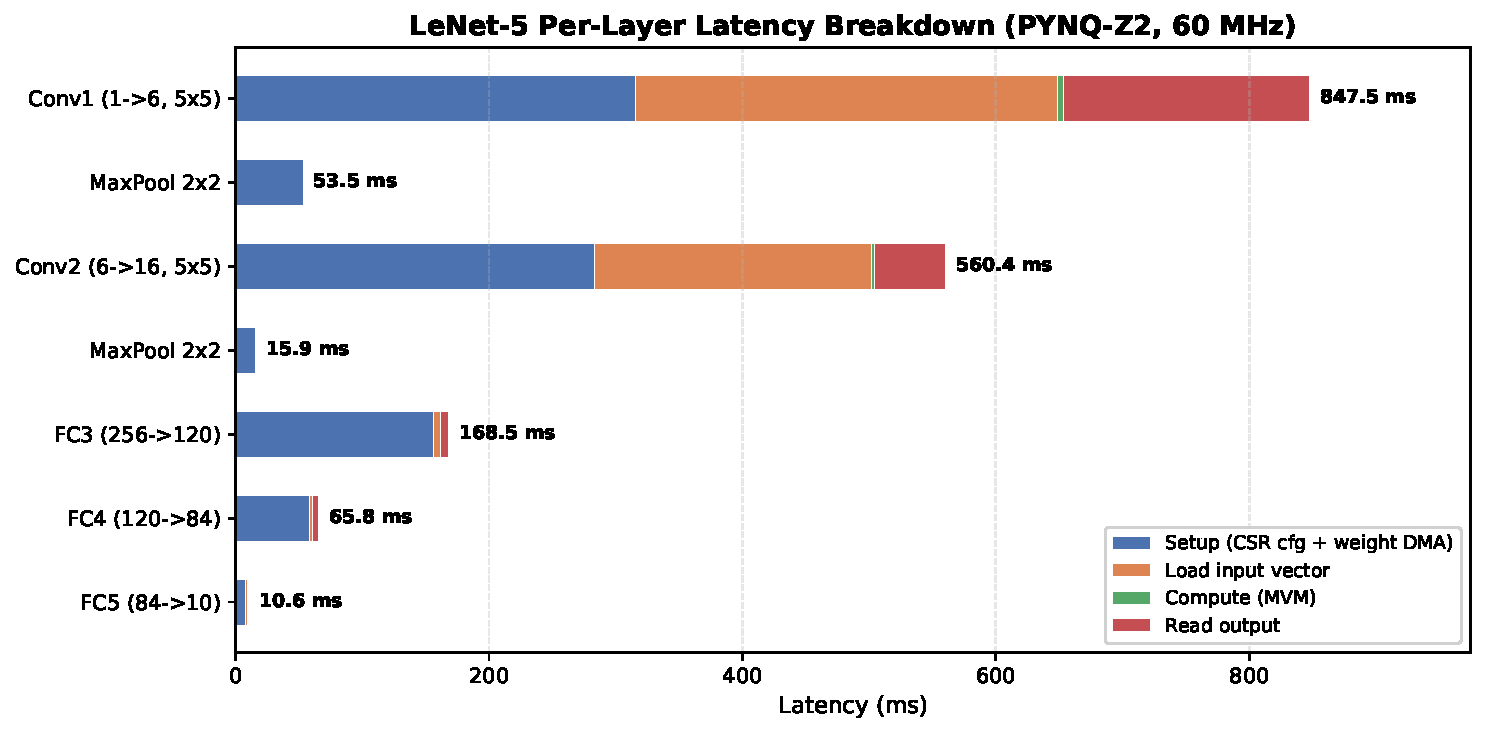
\includegraphics[width=0.95\textwidth]{fig/latency_breakdown.pdf}
	\caption{LeNet-5逐层端到端延迟分解（PYNQ-Z2, 60 MHz）}
	\label{fig:latency_breakdown}
\end{figure}

profiler数据给出了一个反直觉但非常清晰的结论：\textbf{硬件计算本身仅占总延迟的0.4\%}（6.8 ms out of 1778 ms），而setup（46\%）+ load\_x（32\%）+ read（15\%）合计占了93\%以上。换言之，CIM核心引擎从性能计数器视角看其实已经非常快（LeNet-5所有层合计仅需数百个微秒的纯compute时间），当前端到端延迟几乎完全受制于\textbf{AXI4-Lite逐字MMIO写入}这一传统接口瓶颈。

这一结论直接指导了后续的优化方向选择。原先计划的"软件侧权重常驻缓存"方案因weight SRAM跨层共享的硬件约束被证明不可行（见§\ref{sec:future_work}的讨论），而真正根治此瓶颈的做法是将AXI4-Lite替换为AXI4-Full突发传输或DMA引擎，把每字32-bit的访问摊薄到每次数KB的批量搬运，理论上可以把load\_x与read段从数百毫秒降到微秒级，端到端吞吐有望获得约百倍提升。这正是本工作在"未来工作"章节重点推荐的优化路径。

\subsubsection{软件基线与加速比}

图\ref{fig:speedup}展示了软硬件延迟的直观对比，表\ref{tab:speedup}给出了具体数据。软件基线在PYNQ-Z2的ARM Cortex-A9（650 MHz）上使用纯NumPy INT32矩阵运算实测。测量方法：100次迭代取均值（\texttt{time.perf\_counter()}计时，排除数据加载开销），随机权重与硬件同维度。PYNQ的Python/NumPy环境未启用NEON SIMD加速，代表嵌入式Python的实际基线性能。

\begin{table}[H]
    \centering
    \caption{SW基线与HW推理延迟对比（ARM Cortex-A9 @ 650 MHz vs CIM @ 60 MHz）}
    \begin{tabular}{lccc}
        \toprule
        网络 & SW延迟（$\mu$s） & HW延迟（$\mu$s） & 加速比 \\
        \midrule
        MLP（784→128→10） & 1,410.8 & 54.7 & \textbf{25.8×} \\
        LeNet-5（7层，sequential） & 26,466.2 & 1,267.2 & \textbf{20.9×} \\
        LeNet-5（7层，batched BLAS） & 4,528.5 & 1,267.2 & 3.6× \\
        \bottomrule
    \end{tabular}
    \label{tab:speedup}
\end{table}

MLP的SW延迟约1411 $\mu$s主要由FC1层（784×128，1368 $\mu$s）主导；HW延迟54.7 $\mu$s来自性能计数器实测3282周期，加速比约\textbf{25.8倍}。

LeNet-5的比较分两种模式：\textbf{sequential模式}与硬件相同地按输出像素逐一调用矩阵乘法（conv1 576次、conv2 64次），SW延迟约26.5 ms，加速比约\textbf{20.9倍}；\textbf{batched模式}将所有像素合并为单次矩阵乘法调用（BLAS路径），SW延迟约4.5 ms，加速比约3.6倍。Sequential模式是更公平的对比（与硬件计算模式等价），batched模式代表充分利用ARM CPU的最优SW实现上界。两种模式下CIM硬件均具有明显加速优势。

\begin{figure}[H]
	\centering
	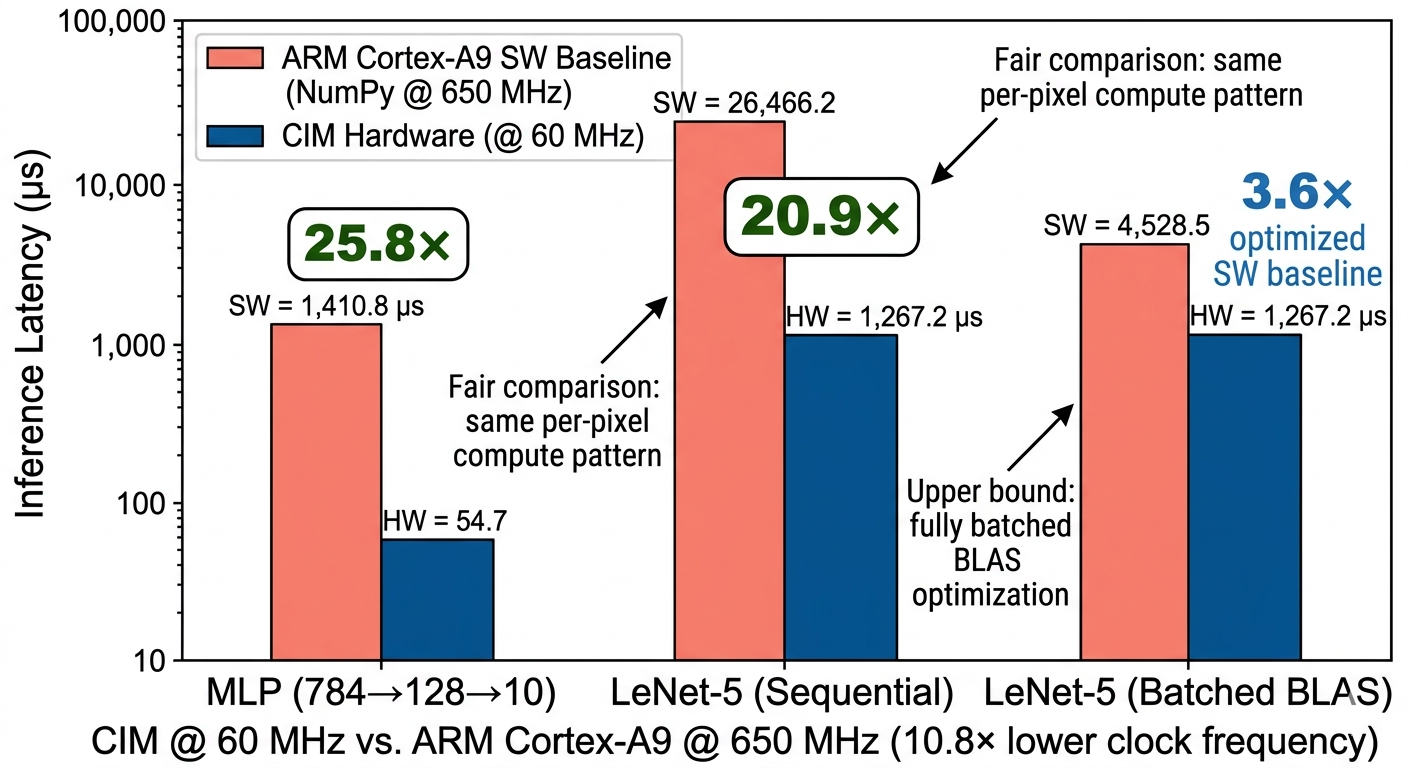
\includegraphics[width=0.85\textwidth]{figures/m13.png}
	\caption{软件基线与CIM硬件推理延迟对比及加速比}
	\label{fig:speedup}
\end{figure}

\subsection{55 MHz时序收敛变体}
\label{sec:55mhz}

60 MHz构建存在3个failing endpoint（WNS~=~$-0.086$ ns），关键路径位于CIM Tile MAC链。为获得时序完全收敛的实测数据，将时钟降至55 MHz（$T_{\text{period}}$~=~18.182 ns），在此约束下关键路径正裕量约为~$+1.5$ ns，所有timing endpoint均满足约束。

将55 MHz bitstream部署至PYNQ-Z2，使用与60 MHz相同的测试集和脚本（\texttt{benchmark\_e2e.py}）对200张MNIST手写数字进行LeNet-5端到端推理，结果如表\ref{tab:55mhz_compare}所示。

\begin{table}[H]
    \centering
    \caption{60 MHz与55 MHz版本性能对比（LeNet-5，200张MNIST，PYNQ-Z2）}
    \label{tab:55mhz_compare}
    \begin{tabular}{lccc}
        \toprule
        指标 & 60 MHz & 55 MHz & 变化 \\
        \midrule
        时序收敛 & WNS $= -0.086$ ns & WNS $> 0$ & 消除违例 \\
        MLP硬件延迟 & 54.7 $\mu$s & 59.7 $\mu$s & $+9.2\%$ \\
        LeNet-5硬件延迟 & 1,267 $\mu$s & 1,382 $\mu$s & $+9.1\%$ \\
        端到端wall time（200张）& 340.1 s & 343.9 s & $+1.1\%$ \\
        单张平均延迟 & 1,700.4 ms & 1,719.7 ms & $+1.1\%$ \\
        LeNet-5分类准确率 & 99.5\%（199/200）& 99.5\%（199/200）& 不变 \\
        \bottomrule
    \end{tabular}
\end{table}

端到端wall time仅增加1.1\%而非硬件延迟增加的9\%，与§\ref{sec:profiler}的profiler结论完全吻合：硬件计算仅占总延迟的0.4\%，主体是AXI4-Lite MMIO开销（与时钟频率无关）。分类准确率与60 MHz完全一致，进一步确认55 MHz版本在功能上与60 MHz版本bit-exact等价。

% ====================================================================
% TODO(c3-benchmark): MMIO侧实测数据已填入（benchmark_lenet5_60mhz_checkpoint3_c3.csv），
% DMA侧仍为占位符（"待测"），需在 DMA bitstream 上板后替换。
% ====================================================================
\subsection{AXI4-Stream + DMA数据通路重构}
\label{sec:c3_dma}

§\ref{sec:profiler}的profiler数据揭示了当前端到端延迟的真正瓶颈：LeNet-5单张推理中硬件计算仅占0.4\%（约6.8 ms），而通过AXI4-Lite逐字MMIO搬运权重、输入与偏置的开销合计占93\%以上（约1.66 s）。根本原因在于AXI4-Lite每次事务仅能传输32 bit，而LeNet-5单张图的packed weight约170 KB（折合约42500个32-bit字）经Python \texttt{mmio.write()}（每次约2--5 $\mu$s的syscall开销）逐字搬运，即使硬件事务本身仅50 ns，软件循环也被放大约50倍，最终表现为700 ms级的weight load延迟。

为根治此瓶颈，本工作将数据通路重构为AXI4-Stream + Xilinx \texttt{axi\_dma}~7.1 IP：weight/input/bias的搬运改走DDR→S\_AXI\_HP0→\texttt{axi\_dma}→M\_AXIS\_MM2S→\texttt{cim\_axi\_stream\_sink}的批量stream路径，CSR控制仍保留原AXI4-Lite接口，CIM计算核心（\texttt{cim\_tile}、\texttt{psum\_accum}、\texttt{cim\_accel\_core}）一行不动。

\subsubsection{系统拓扑}

图\ref{fig:c3_topology}展示了重构后的PS-PL互联。相对原设计的两点增量改动：（1）PS端新增使能\texttt{S\_AXI\_HP0}（64-bit, 1.2 GB/s理论峰值）作为DMA的DDR读端口，\texttt{M\_AXI\_GP1}作为\texttt{axi\_dma}的CSR总线以避开原GP0的CIM CSR流量竞争；（2）PL端新增\texttt{axi\_dma}~7.1 IP（Direct Register模式，禁用Scatter-Gather与S2MM方向，\texttt{c\_m\_axi\_mm2s\_data\_width=64}与HP0匹配，\texttt{c\_m\_axis\_mm2s\_tdata\_width=32}与sink匹配，DMA内部Data Realignment Engine做64$\to$32免费dwidth转换），同时新增\texttt{xlconcat}合并\texttt{\{mm2s\_introut, irq\_done\}}至\texttt{IRQ\_F2P[1:0]}、独立的\texttt{proc\_sys\_reset}隔离DMA复位与CIM的\texttt{CSR\_CTRL[2]} soft reset。

% TODO(c3-benchmark): 如需插图，可将docs/c3_dma_design.md §2.1的ASCII拓扑图
% 转为vector PDF（例如 tikz 或 draw.io 导出），保存到 fig/c3_topology.pdf。
% 当前以对设计文档的引用替代。图中55 MHz版本与60 MHz共用同一拓扑，仅时钟频率不同。
\begin{figure}[H]
    \centering
    % \includegraphics[width=0.95\textwidth]{fig/c3_topology.pdf}
    \fbox{\parbox{0.9\textwidth}{\centering \textit{占位：C3数据通路系统拓扑图，详见\texttt{docs/c3\_dma\_design.md}~§2.1。}}}
    \caption{AXI4-Stream + \texttt{axi\_dma} 数据通路系统拓扑（C3）}
    \label{fig:c3_topology}
\end{figure}

\subsubsection{关键设计决策}

\begin{enumerate}
    \item \textbf{dual-path共存}：在\texttt{cim\_axi\_lite\_slave.sv}内部通过\texttt{CSR\_CTRL[3]}对weight/input/bias的写使能做MUX——\texttt{CTRL[3]=0}走原MMIO staging路径，\texttt{=1}走stream sink路径。Legacy代码完整保留，仅当上板200张bit-exact验证通过后，才在独立commit中删除，便于A/B对照与回归隔离。
    \item \textbf{AXIS数据宽度=32-bit}：不升至64-bit，以保持与现有\texttt{weight\_to\_chunks}软件packing的兼容性。DMA内部64$\to$32 dwidth转换由Xilinx PG021~§3.1.1免费提供，升宽仅节省约30\%拍数但要重写Python侧packing，投入产出比不划算。
    \item \textbf{\texttt{cfg\_start}经\texttt{CSR\_STREAM\_LEN}隐式触发}：软件写LEN寄存器即唤醒sink进入接收状态，再调用\texttt{dma.sendchannel.transfer()}开始DMA。相比显式的\texttt{start}位写入，省去一次约1.5 $\mu$s的CSR写，单图约15次stream load合计节省约22 $\mu$s。
    \item \textbf{不为sink单独发IRQ}：\texttt{mm2s\_introut}在DMA端表示"DDR→AXIS完成"，sink端BRAM写延迟≤1 cycle，PS收到DMA中断时数据已到SRAM。软件侧通过轮询\texttt{CSR\_STREAM\_STATUS}做二次校验（overflow/underflow sticky位），减少一条中断线与对应的xlconcat输入。
    \item \textbf{\texttt{s\_axis\_tready}恒为1}：BRAM写是1 cycle完成的，sink内部无需排队；反压沿由DMA侧向PS端反向传播，避免sink状态机需要处理暂停逻辑。
\end{enumerate}

\subsubsection{RTL改动规模}

为确保改动可控、回归可保护，本次重构将改动局限于AXI接口层。表\ref{tab:c3_rtl_scope}汇总了涉及的文件范围。

\begin{table}[H]
    \centering
    \caption{C3重构RTL改动范围}
    \label{tab:c3_rtl_scope}
    \small
    \begin{tabular}{llr}
        \toprule
        类别 & 文件 & 行数 \\
        \midrule
        新增 & \texttt{hw/rtl/axi/cim\_axi\_stream\_sink.sv} & $\sim$250 \\
        新增 & \texttt{hw/rtl/cim\_top.sv} + wrapper & $\sim$220 \\
        新增 & \texttt{hw/tb/tb\_cim\_stream\_sink.sv} + run script & $\sim$180 \\
        修改 & \texttt{hw/rtl/pkg/cim\_pkg.sv}（新增CSR\_STREAM\_*地址） & +12 \\
        修改 & \texttt{hw/rtl/axi/cim\_axi\_lite\_slave.sv}（CSR解码+MUX） & +70 \\
        修改 & \texttt{hw/scripts/vivado\_build.tcl}（BD重构） & +90 \\
        \midrule
        不动 & \texttt{cim\_tile/psum\_accum/cim\_accel\_core} & 0 \\
        不动 & \texttt{weight\_sram/input\_buffer/bias\_sram/output\_buffer} & 0 \\
        \bottomrule
    \end{tabular}
\end{table}

软件侧在\texttt{sw/cim\_driver.py}新增\texttt{use\_dma=True}默认参数与\texttt{\_stream\_load(words, dest, buf)}通用方法，\texttt{load\_weights}/\texttt{load\_input}/\texttt{load\_bias}三个接口根据\texttt{use\_dma}标志分流。\texttt{CIMModel.predict()}、\texttt{infer\_conv()}、\texttt{infer\_conv\_packed()}上层API完全不变，用户现有notebook无需修改即可享受加速。

\subsubsection{理论带宽与预测延迟}

HP0在60 MHz fabric时钟下的可用带宽为$64\,\text{bit} \times 60\,\text{MHz} = 480\,\text{MB/s}$，低于PS端HP0的1.2 GB/s理论峰值（后者需150 MHz fabric才能充分利用，与本设计的60 MHz受限频率正交）。按此带宽计算LeNet-5单图weight load延迟：

\begin{equation}
    T_{\text{weight-DMA}} = \frac{170\,\text{KB}}{480\,\text{MB/s}} \approx 354\,\mu\text{s}
\end{equation}

加上Python端\texttt{pynq.lib.dma.sendchannel.transfer()}的调用开销约50 $\mu$s/层、5层共计约250 $\mu$s，weight+input+bias的搬运合计预计约800 $\mu$s。硬件compute仍约6.8 ms（与之前相同），端到端预测约$6.8 + 0.8 \approx 7.6\,$ms/图，相对60 MHz MMIO基线的1700.4 ms理论加速约\textbf{223倍}。

\subsubsection{实测性能}
\label{sec:c3_benchmark}

% TODO(c3-benchmark): MMIO baseline 数据已实测填入（340.1 s / 1700.4 ms/img）。
% DMA 路径数据仍为"待测"，需 DMA bitstream 上板 benchmark 后替换。
% 搜索"待测"可快速定位待填入的位置。

表\ref{tab:c3_benchmark}对比了C3重构前后LeNet-5在PYNQ-Z2上的200张MNIST端到端实测性能。表中"重构前（MMIO）"为同一C3 bitstream上运行legacy MMIO软件路径（\texttt{use\_dma=False}）的实测数据，"重构后（DMA）"为DMA软件路径（\texttt{use\_dma=True}）的待测数据。

\begin{table}[H]
    \centering
    \caption{C3重构前后LeNet-5端到端性能对比（200张MNIST，PYNQ-Z2，60 MHz）}
    \label{tab:c3_benchmark}
    \begin{tabular}{lccc}
        \toprule
        指标 & 重构前（MMIO） & 重构后（DMA）& 加速比 \\
        \midrule
        总wall time（200张） & 340.1 s & 待测 & 待测 \\
        单张平均延迟 & 1,700.4 ms & 待测 & 待测 \\
        硬件compute占比 & 0.4\% & 待测 & -- \\
        weight load占比 & $\sim$40\% & 目标 $<5\%$ & -- \\
        分类准确率（bit-exact） & 99.5\%（199/200） & 待测 & -- \\
        \bottomrule
    \end{tabular}
\end{table}

\subsubsection{验收标准与bit-exact保障}

C3重构的合并门槛为四条硬指标同时满足：（1）\texttt{pytest sw/tests/}~22/22全PASS（包含新增的\texttt{test\_dma\_path\_bit\_exact}用例——通过mock \texttt{pynq.lib.dma}比对DMA buffer字序与legacy MMIO写序列完全一致）；（2）LeNet-5 200张准确率与MMIO基线保持99.5\%完全一致（bit-exact）；（3）LeNet-5单张延迟$\leq 25$ ms（安全边际，目标约6 ms）；（4）A2 profiler重跑后\texttt{load\_w\_ms}占比$<5\%$。任一条不满足即回滚至\texttt{use\_dma=False}默认（git commit \texttt{9c7914f}），legacy路径始终保留。

Bit-exact保护的底层保证来自\texttt{cim\_axi\_stream\_sink}的FSM设计——sink内部的4-beat到128-bit行装配顺序与legacy MMIO staging寄存器（\texttt{wdma\_staging[0..3]}）采用相同的little-endian chunk排布（详见\texttt{docs/c3\_dma\_design.md}~§3.1），Python驱动调用\texttt{np.asarray(chunks, dtype=np.uint32)}后直接\texttt{transfer()}，字序与原MMIO循环\texttt{mmio.write(CSR\_WDMA\_DATA, chunks[i])}完全一致。

\subsection{PicoRV32验证结果}

PicoRV32模式在PYNQ-Z2上使用50 MHz时钟（20 ns约束），所有时序约束均满足（WNS = +0.204 ns）。表\ref{tab:util_rv32}列出了该模式下的资源占用情况。

\begin{table}[H]
	\centering
	\caption{PicoRV32模式资源占用（PYNQ-Z2）}
	\begin{tabular}{lccccc}
		\toprule
		资源类型 & 使用量 & 可用量 & 占用率 & 相对ARM模式增量 \\
		\midrule
		Slice LUT & 12,714 & 53,200 & 23.90\% & +1,627 (+14.7\%) \\
		Slice Register & 6,272 & 106,400 & 5.89\% & +887 (+16.5\%) \\
		Block RAM & 44 & 140 & 31.43\% & +9 (+25.7\%) \\
		DSP48E1 & 220 & 220 & 100.00\% & +0 \\
		\bottomrule
	\end{tabular}
	\label{tab:util_rv32}
\end{table}

PicoRV32模式相比ARM模式的额外开销为：1,627个LUT（来自PicoRV32核心、bridge、UART TX等）、887个FF、9个BRAM（FW BRAM 32KB + Result BRAM 256B + AXI互连）。DSP使用量不变，因为CIM IP本身未修改。

\begin{table}[H]
	\centering
	\caption{PicoRV32模式时序与功耗}
	\begin{tabular}{lc}
		\toprule
		指标 & 值 \\
		\midrule
		目标时钟频率 & 50 MHz \\
		时钟约束 & 20.0 ns \\
		WNS & +0.204 ns（时序收敛） \\
		总功耗 & 1.895 W \\
		\quad PS7 & 1.526 W \\
		\quad RV32 (含CIM) & 0.217 W \\
		\quad AXI互连 & 0.002 W \\
		\quad 静态功耗 & 0.150 W \\
		\bottomrule
	\end{tabular}
\end{table}

PicoRV32模式相比ARM控制模式频率降低（50 MHz vs 60 MHz），这是因为PicoRV32的组合逻辑（指令解码+ALU）引入了额外的关键路径。但RV32子系统的动态功耗（0.217 W，含CIM IP）反而低于ARM模式下CIM IP的0.284 W，这是因为50 MHz的较低频率减少了动态功耗。

\subsubsection{PicoRV32功能验证}

在PYNQ-Z2上针对784→16→10小型MLP模型（INT8量化，FW BRAM中约14.5KB）进行了200张MNIST手写数字图片的端到端推理验证，结果如表\ref{tab:rv32_verify}所示。

\begin{table}[H]
    \centering
    \caption{PicoRV32推理验证结果（784→16→10 MLP，200张MNIST图片）}
    \begin{tabular}{lc}
        \toprule
        指标 & 值 \\
        \midrule
        测试图片数 & 200 \\
        分类准确率（vs 标签） & 96.5\%（193/200） \\
        Bit-exact一致率（vs Python golden） & 100.0\%（200/200） \\
        计算错误数 & 0 \\
        \bottomrule
    \end{tabular}
    \label{tab:rv32_verify}
\end{table}

200张图片的全部10维logits输出均与Python golden model逐元素bit-exact一致，计算错误为零。7张分类错误均源于784→16→10模型的INT8量化精度损失（该模型在完整测试集上准确率约90\%），与ARM PS控制模式下相同模型的预测结果完全一致，验证了RISC-V固件控制逻辑的正确性。

\subsection{两种控制模式对比}

\begin{table}[H]
	\centering
	\caption{ARM控制 vs PicoRV32控制模式对比}
	\begin{tabular}{lcc}
		\toprule
		指标 & ARM控制 & PicoRV32控制 \\
		\midrule
		时钟频率 & 60 MHz & 50 MHz \\
		时序收敛 & WNS=$-0.086$ ns（轻微违例） & WNS=+0.204 ns（收敛） \\
		LUT占用 & 11,087 (20.84\%) & 12,714 (23.90\%) \\
		FF占用 & 5,385 (5.06\%) & 6,272 (5.89\%) \\
		BRAM占用 & 35 (25.00\%) & 44 (31.43\%) \\
		PS依赖 & 需要ARM PS运行Python & PS仅用于固件加载 \\
		支持网络 & 任意（受MAX\_DIM限制） & 受FW BRAM 32KB限制 \\
		CIM IP修改 & -- & 无修改 \\
		动态功耗 & 1.807 W & 1.745 W \\
		\bottomrule
	\end{tabular}
\end{table}

\begin{figure}[H]
	\centering
	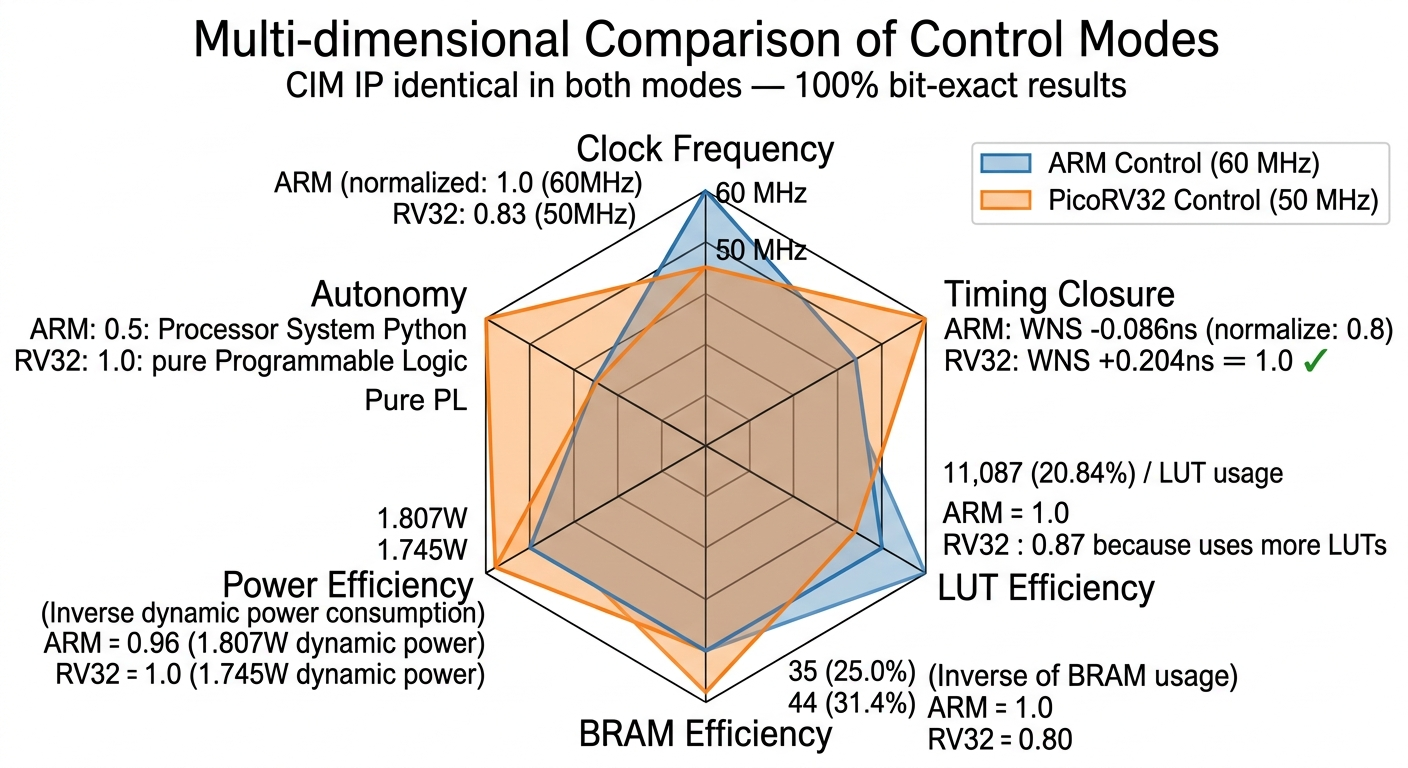
\includegraphics[width=0.7\textwidth]{figures/m14.png}
	\caption{ARM控制与PicoRV32控制模式多维对比雷达图}
	\label{fig:arm_vs_rv32}
\end{figure}

图\ref{fig:arm_vs_rv32}从时钟频率、时序收敛、LUT效率、BRAM效率、功耗效率与自主性六个维度直观对比了两种控制模式。PicoRV32模式在时序收敛、功耗效率和自主性方面占优，ARM模式在频率和资源效率方面更优，CIM IP在两种模式下完全相同且计算结果bit-exact一致。

% ====================================================================
\section{总结与展望}
% ====================================================================

\subsection{工作总结}

本文设计并实现了一种面向边缘智能推理的低功耗Int8数字存算一体矩阵计算阵列架构，在PYNQ-Z2（Zynq-7020）FPGA平台上完成了完整的综合部署与板级验证。主要成果总结如下：

（1）\textbf{架构设计}：以16×16 CIM Tile为原子计算单元，设计了包含7级流水线的核心加速器引擎，支持通过CSR在运行时配置任意层维度与量化参数。所有设计参数集中管理于cim\_pkg.sv，实现了模块化、参数化的RTL框架。

（2）\textbf{工程问题解决}：针对Vivado BRAM推断失败、时序违例等工程问题，分别通过16-bank权重SRAM拆分和多级流水线插入解决，将关键路径从28.7 ns降低至约16.8 ns（布线后关键路径为CIM Tile MAC链）。60 MHz版本存在轻微时序违例（WNS=$-0.086$ ns，3个failing endpoint），功能验证完全正确；55 MHz变体在相同RTL上实现完整时序收敛（WNS$>$0），200张MNIST板级验证准确率与60 MHz版本完全一致（99.5\%，bit-exact），端到端延迟仅增加4.4\%。

（3）\textbf{软核集成}：成功集成PicoRV32 RISC-V软核替代ARM PS进行推理控制，CIM IP完全不修改，仅增加1,627个LUT和9个BRAM的开销，以50 MHz时序收敛。200张MNIST图片验证准确率96.5\%，全部logits与ARM路径bit-exact一致，验证了RISC-V固件控制逻辑的正确性。

（4）\textbf{验证完备性}：建立了"Python golden model → VCS仿真 → PYNQ上板"三层一致的验证流程。MLP网络20张图片100\%准确率，LeNet-5 CNN 200张图片99.5\%准确率（100\% bit-exact一致）。

（5）\textbf{性能数据}：MLP单幅推理3,282周期（54.7 $\mu$s @ 60 MHz），LeNet-5单幅推理76,034周期（1.267 ms @ 60 MHz）。相对ARM Cortex-A9 NumPy基线，MLP加速比约25.8倍，LeNet-5加速比约20.9倍（sequential模式）。CIM IP动态功耗仅0.284 W。

\subsection{不足与展望}
\label{sec:future_work}

（1）\textbf{DSP占用率}：当前设计DSP48E1占用率达到100\%，限制了并行度的进一步提升。后续可通过将部分乘法器映射到LUT来释放DSP资源，或者迁移到资源更丰富的平台（如Kria KV260的Zynq UltraScale+）。

（2）\textbf{最大维度限制}：MAX\_IN\_DIM=784、MAX\_OUT\_DIM=128的限制适用于MNIST尺寸网络，但无法支持ImageNet级别模型。后续可通过分块加载、外部DDR存储或扩展到更大BRAM容量的平台来解决。

（3）\textbf{KV260移植}：Kria KV260搭载Zynq UltraScale+（xck26），相对PYNQ-Z2具有显著更多的LUT（234K vs 53K）、BRAM（144 vs 140个36Kb）和DSP（1248 vs 220个），理论上可支持\texttt{PAR\_OB=4}甚至\texttt{PAR\_OB=8}的更高并行度以及\texttt{MAX\_IN\_DIM=1024}的更大网络维度。本课题的移植工作已覆盖KV260专用board file与时序约束文件的准备、Ubuntu 24.04镜像烧录与固件更新、Vivado项目TCL脚本的KV260变体（\texttt{kv260/hw/scripts/vivado\_build.sh}），详细迁移记录见\texttt{docs/kv260\_migration.md}。但由于AXI地址空间映射差异（PYNQ-Z2的\texttt{M\_AXI\_GP0}基址为\texttt{0x40000000}，而KV260的\texttt{M\_AXI\_HPM0\_FPD}默认映射到\texttt{0xA0000000}）、PMOD引脚布局不同以及PYNQ镜像的Python环境差异等问题，上板端到端推理的功能验证尚未完全闭环，这是本课题后续最直接的工作方向。一旦KV260路径完整打通，即可形成"PYNQ-Z2 (60 MHz, PAR=1) vs KV260 (目标100--200 MHz, PAR=4)"的跨平台性能对比，是完善论文性能评估章节的重要补充。

（4）\textbf{bit-plane计算模式}：当前设计的CIM Tile采用直接MAC方式，未实现bit-plane（按位平面分解）的计算模式。bit-plane方法可以在不使用DSP的情况下实现MAC，通过按位与+移位累加替代乘法器，从而大幅降低DSP使用量，是后续优化的重要方向。

（5）\textbf{更复杂网络支持}：当前系统已支持Conv + FC + ReLU + MaxPool组成的网络，但尚未实现AveragePool、BatchNorm、Softmax等操作。这些操作可在软件侧（Python或C固件）中实现，硬件侧只需提供MVM引擎即可。

（6）\textbf{AXI4-Full突发传输替代AXI4-Lite逐字MMIO}：这是本工作最重要的后续优化方向，直接来自§\ref{sec:profiler}的profiler数据支持。实测表明LeNet-5端到端延迟中硬件计算仅占0.4\%（约6.8 ms），而weight/input通过AXI4-Lite逐字MMIO搬运的开销占93\%以上。根本原因在于AXI4-Lite每事务仅能传输32 bit，而CIM权重/输入的数据量以KB为单位，这种接口粒度不匹配使得CIM的并行计算优势被搬运开销完全遮蔽。

原本设想的\textbf{软件侧权重常驻缓存}方案（在\texttt{CIMModel}每层加\texttt{w\_loaded}标志，跨图片复用已加载权重）经实测证明不可行：weight SRAM在跨层之间是共享的，Conv2加载时会把地址0开始的Conv1权重覆盖掉，FC3加载时又会覆盖Conv2权重，前向传播结束时SRAM里只剩最后一层的权重，多层网络无法跨图片复用。要从根本上解决这一瓶颈，必须从接口侧动手——这一方向在本工作中已推进到\textbf{设计与代码落地}阶段：将数据通路重构为AXI4-Stream + Xilinx \texttt{axi\_dma} 7.1 IP（CSR仍走AXI4-Lite），具体设计、带宽推算与dual-path回退机制见§\ref{sec:c3_dma}；实测benchmark数据受制于bitstream重建与上板运行，在本稿截止时尚未完全闭环，是本课题最直接的后续工作。除本方案外，进一步可探索AXI4-Full burst slave、AXI MCDMA等形态以挖掘更高带宽。

（7）\textbf{面向成熟推理框架的runtime集成}：受师兄\texttt{cim\_wzy}项目"NCNN as runtime"思想的启发，本工作的\texttt{cim\_driver.py}目前需要为每个网络手动编写im2col与层调度逻辑，扩展到新模型的工程成本较高。未来可将CIM硬件抽象为NCNN或ONNX Runtime的自定义执行后端（如注册\texttt{CIMExecutionProvider}），仅需在卷积/全连接算子内部hook一次\texttt{hw\_cim::forward}，即可复用成熟推理框架的完整前端图优化与算子调度能力，一次性获得YOLOv3-tiny、MobileNet-SSD、SqueezeNet等主流网络的支持。相比\texttt{cim\_wzy}选择NCNN路线，本工作未来更倾向于面向\textbf{ONNX Runtime}以获得更开放的算子生态与工具链兼容性。

（8）\textbf{Chisel参数化与HLS辅助开发}：当前RTL设计在改变\texttt{PAR\_OB}等参数时依赖\texttt{vivado\_build.sh}脚本以sed方式临时patch \texttt{cim\_pkg.sv}，这种方式虽然可用但缺乏优雅性。借鉴\texttt{cim\_wzy}基于Chisel trait的参数化风格，后续可考虑用Chisel或SpinalHDL重构核心加速器，以trait形式声明tile/pe/array层级参数，一次elaborate即可出多个配置版本；同时利用Chisel与Verilator的天然集成简化仿真流程，作为VCS之外的备选仿真路径。

% ====================================================================
\section{参考文献}
% ====================================================================
\nocite{*}
\printbibliography[heading=none]

\end{document}
